%-----------------------------------------------------------------------------
%
%               Template for sigplanconf LaTeX Class
%
% Name:         sigplanconf-template.tex
%
% Purpose:      A template for sigplanconf.cls, which is a LaTeX 2e class
%               file for SIGPLAN conference proceedings.
%
% Guide:        Refer to "Author's Guide to the ACM SIGPLAN Class,"
%               sigplanconf-guide.pdf
%
% Author:       Paul C. Anagnostopoulos
%               Windfall Software
%               978 371-2316
%               paul@windfall.com
%
% Created:      15 February 2005
%
%-----------------------------------------------------------------------------


\documentclass{sigplanconf}

% The following \documentclass options may be useful:

% preprint      Remove this option only once the paper is in final form.
% 10pt          To set in 10-point type instead of 9-point.
% 11pt          To set in 11-point type instead of 9-point.
% authoryear    To obtain author/year citation style instead of numeric.

\usepackage{amsmath}
\usepackage{graphicx}
\usepackage{subfig}


\begin{document}

\special{papersize=8.5in,11in}
\setlength{\pdfpageheight}{\paperheight}
\setlength{\pdfpagewidth}{\paperwidth}

\conferenceinfo{CONF 'yy}{Month d--d, 20yy, City, ST, Country} 
\copyrightyear{20yy} 
\copyrightdata{978-1-nnnn-nnnn-n/yy/mm} 
\doi{nnnnnnn.nnnnnnn}

% Uncomment one of the following two, if you are not going for the 
% traditional copyright transfer agreement.

%\exclusivelicense                % ACM gets exclusive license to publish, 
                                  % you retain copyright

%\permissiontopublish             % ACM gets nonexclusive license to publish
                                  % (paid open-access papers, 
                                  % short abstracts)

\titlebanner{banner above paper title}        % These are ignored unless
\preprintfooter{short description of paper}   % 'preprint' option specified.

\title{Title Text}
\subtitle{Subtitle Text, if any}

\authorinfo{Name1}
           {Affiliation1}
           {Email1}
\authorinfo{Name2\and Name3}
           {Affiliation2/3}
           {Email2/3}

\maketitle

\begin{abstract}
    The emergence of dynamic multicore systems allows for new hardware
    optimisations where hardware modifies itself to match the software's needs.
    In this paper we describe an automatic method of determining how to
    partition a program and associate each partition to a set of fused cores in
    order  to improve the performance of streaming applications through the use
    of machine learning. We explore the difficulties of extracting important
    features out of programs in order to accurately decide the correct chip
    topology.  Using the methods described in the paper we can achieve up to 2
    times speedup on certain applications.
\end{abstract}

\category{CR-number}{subcategory}{third-level}

% general terms are not compulsory anymore, 
% you may leave them out
\terms
term1, term2

\keywords
keyword1, keyword2

\section{Introduction}
% Software point of view: the problem
A Dynamic Multicore Processor's (DMP) ability to reconfigure itself allows it to adapt to any program it executes.
Whilst being able to reconfigure hardware is a promising approach to optimising execution, DMPs come with their own set of challenges when attempting to finding a good configuration for the program at hand.
Given a program that can be parallelised, a DMP can either be configured to run a high number of threads on small groups of cores, a small number of threads on large groups of cores or a heterogeneous mix of both large and small cores.
Without deep knowledge of the architecture, knowing what configuration of the processor is correct in order to be able to obtain the best performance, can be a highly time consuming task.
This is due to the fact that determining the configuration can require multiple profiling passes if the configuration count is high, and this task will have to be repeated whenever significant modifications to the program are made.
This can be further complicated if the programming model does not provide any insights on how the program may be partitioned into threads.
The problem of optimising multi-threaded software for DMPs can therefore be split into two distinct tasks.
First, finding a programming model that makes software partitioning into threads explicit.
Second, using information from both the hardware and software, automate the partitioning of both the software into threads, and the hardware into compositions.

In most parallel programming models, such as OpenMP~\cite{openmp}, the user is directly responsible for mapping parallelism to the hardware; a difficult and time consuming task~\cite{prabhu2011LanguagePar}.
This is due to the fact that these models extend programming languages that do not consider parallelism as a defining design factor~\cite{pingaliTao2011}.
On the other-hand, dataflow programming models such as StreamIt~\cite{theis2002streamit} and Lime \cite{auerbach2012lime} make data and parallelism first class citizens.
In these languages, applications are expressed as data oriented graphs and --- ideally --- the compiler or runtime determines the mapping of parallelism onto the available hardware and controls the grouping of hardware resources.
Thus using such a model can be a potential solution to the first part of the problem.

However, optimally mapping parallelism and managing hardware resources remains an open problem given the sheer complexity of the resulting design space.
For example, given a 16 core DMP with up to 15 threads, a program can have over 32,000 different configurations of thread to core composition pairings.
Rather than exhaustively searching the space, which is a very time consuming task, finding a way to automate the configuration of the processor makes using DMPs more attractive.
The number of program features that may influence how to partition programs is large, for example it could depend on the number of tasks, the parallelism made explicit by the language and/or different compiler optimisations.
Therefore manually determining a set of heuristics to create a model that selects thread count and core compositions is not recommended as important information may be disregarded.
Instead, correlation analysis is used to determine which features, from a set of handpicked features, correlate the most with deciding a good partition and are to be used to generate an appropriate machine learning model.

This chapter analyses how static ahead-of-time reconfiguration of a DMP can improve performance of a set of streaming applications.
In this setting, static defines a core composition that does not change during the execution of a program, whilst ahead of time means the configuration is set before execution.
These streaming applications include audio signal and image processing and sorting algorithms.
Streaming programs are ubiquitous in the embedded systems space~\cite{theis2002streamit} and their mix of parallelism and computation make them an interesting domain for DMPs.

An analysis of the design space is performed and shows the impact of modifying resources and thread mapping and is conducted using a set of StreamIt programs.
A machine learning model is developed using the information gathered from the exploration.
This model predicts the best number of threads for a given application and an optimal number of cores to allocate to each thread.
To demonstrate the viability of the approach the results of the predictive model are compared to the best sampled thread and core composition pairing in a space of more than 32,000 design points.
The model can match the performance of the best sampled points, with speedups of up to 9x on a 16 core processor compared to single-threaded execution on a single core. 

% contributions
The main contributions of this chapter are:
\vspace{-1em}
\begin{itemize}
\item An analysis of the co-design space of thread partitioning and core composition;
\vspace{-1em}
\item A study on the impact of a loop transformation on the optimal core composition;
\vspace{-2em}
\item A machine-learning model that determines the optimal core composition and thread partitioning ahead of time in order to get the optimal performance;
\vspace{-1em}
\item An analysis of the static code features that are considered the most important for determining a correct configuration of the system by the model.
\end{itemize}


The chapter is structured as follow,
Section~\ref{sec:motiviation-str} motivates this work by showing the complexity of the design space.
Section~\ref{chp:stream:sec:setup} describes the methodology and section~\ref{sec:streamit:dse} presents an in-depth analysis of the design space.
Section~\ref{sec:ml} develops a machine-learning model to predict the best thread mapping and core composition whilst section~\ref{sec:results} shows the performance of the model.
Section~\ref{sec:conclusion} concludes this chapter.

%In most parallel programming models such as OpenMP, the user is directly responsible for mapping parallelism to the hardware; a difficult and time consuming task.
%This problem is further exacerbated when hardware resources can be combined since programmers have to take into account the dynamic behavior of the architecture~\cite{bower2008impactd}.

% Solution for the software: data flow programming
%To solve this problem, this chapter demonstrates that there is a need to raise the programming abstraction and remove the burden of mapping parallelism from programmers.
%Dataflow programming models such as StreamIt~\cite{theis2002streamit} and Lime~\cite{auerbach2012lime} offer one part of the solution.
%Applications are expressed as dataflow graphs and --- ideally --- the compiler or runtime determines the mapping of parallelism onto the available hardware and controls the grouping of hardware resources.
%However, optimally mapping parallelism and managing hardware resources remains an open problem given the sheer complexity of the resulting design space.

% What we do: 1st an analysis


\section{Motivation}
\begin{figure}[t]
    \centering
    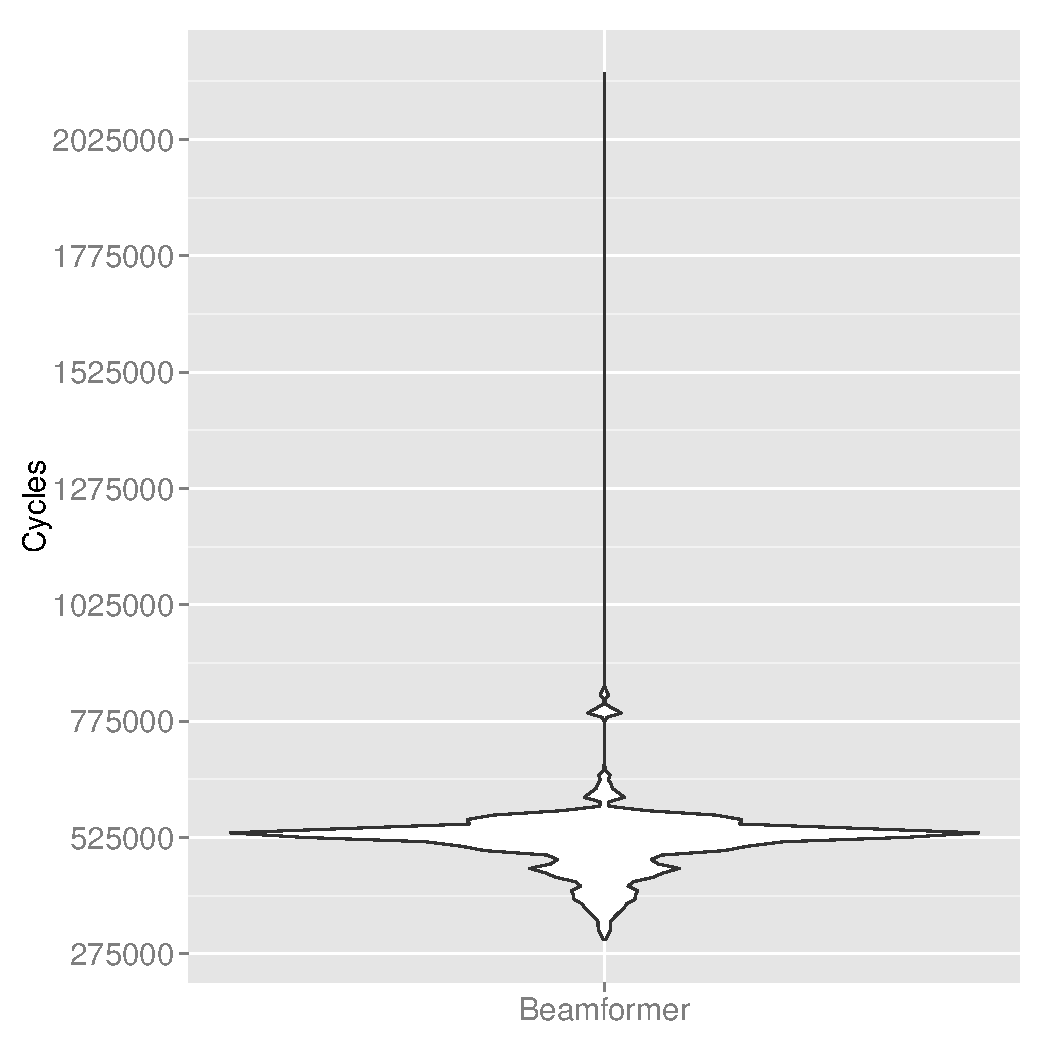
\includegraphics[width=1\textwidth]{streamit-paper/graphics/beamformer_motivation.pdf}
    \caption{Distribution of the runtime for Beamformer resulting from an exhaustively exploration of the hardware/software co-design space.
     The application has been partitioned into different number of threads and core compositions.}
     \label{fig:beamformermotiv}
\end{figure}

This section illustrates the difficulty of finding a good partition and resource allocation.
A simple experiment is conducted where one StreamIt benchmark is taken, \bench{Beamformer}, and partition its tasks into threads and allocate various number of cores to each thread.
A co-design of more than 32,000 combinations (exhaustive space) of thread mappings and core compositions is generated.
Each design point is executed on a dynamic multicore simulator (exact details about the experimental setup are presented later in section~\ref{sec:setup}).

Figure~\ref{fig:beamformermotiv} presents the distribution of the execution times from the co-design space as a violin plot.
For the unfamiliar reader, an intuitive way to think about this violin plot is to consider it as a smoothed histogram rotated by 90 degrees and mirrored.
The majority of the sampled points have a cycle count around 525,000 with the worst points taking more than 2 millions cycles.
The best performance is around 275,000 cycles which is about 2x faster than the majority of the data points.
This shows that finding the right combination of thread mapping and core composition is critical since a wrong choice often leads to suboptimal performance.

This example illustrates the necessity for designing the technique to predict both the optimal number of threads and core composition to use.
The next section will present a more in-depth analysis of the design space before presenting our machine-learning predictive model.



\section{Background}
\chapter{Background}
This chapter covers the different topics that are present in this thesis.
The background starts by briefly covering Chip Multicore Processors and Heterogeneous Chip Multicore Processors to motivate the existence of Dynamic Multicore Processors.
Then the core-fusion technique, which is the main mechanism brought forward by Dynamic Multicore Processors is described in detail.
This is followed by a description of the EDGE instruction set architecture which is used in the Dynamic Multicore Processor described in this thesis.
Finally, streaming programming languages, which are used in Chapter~ref{}, are explained.

\section{Chip Multicore Processors}

\begin{figure}[t]
 \center
 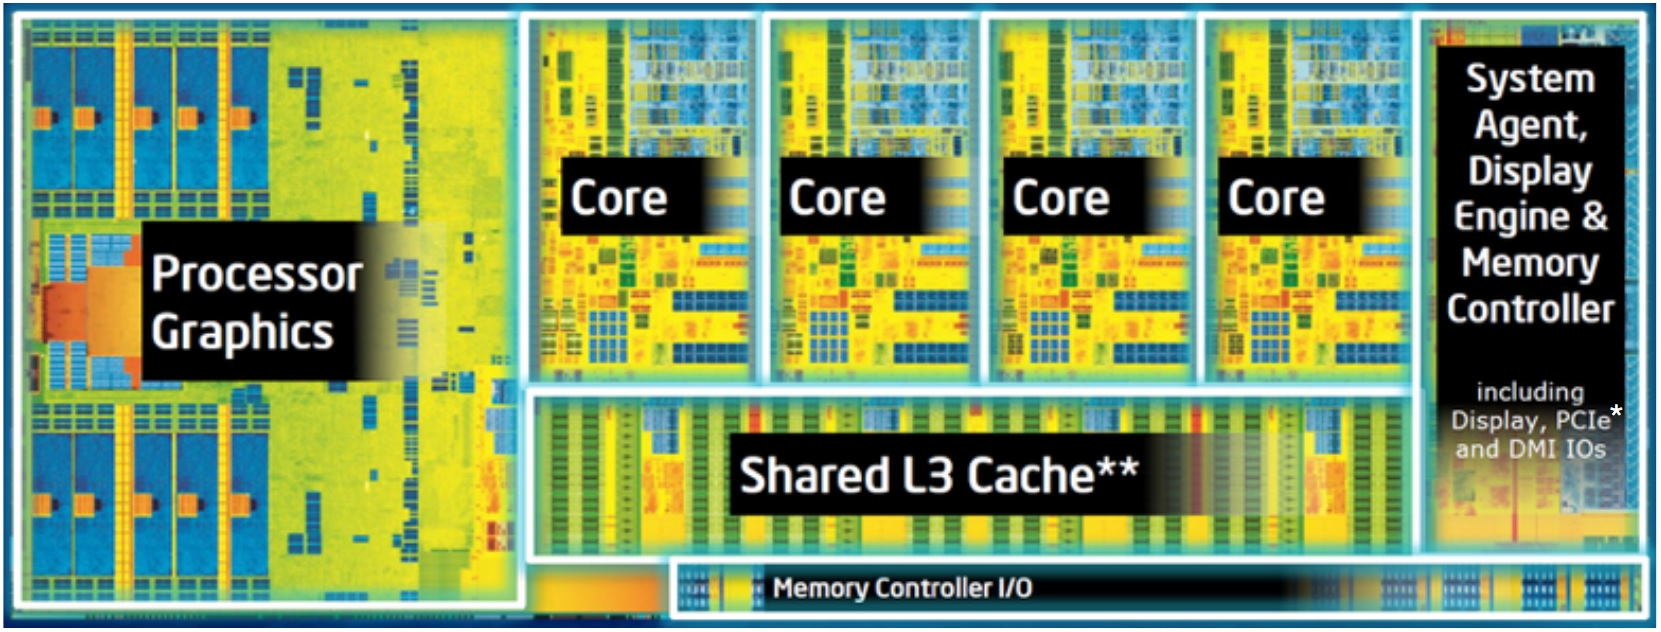
\includegraphics[width=1\textwidth]{background/graphics/i7intel.jpg}
 \caption{Intel Core i7 processor internal die photograph taken from intel whitepaper}\label{fig:i7}
\end{figure}
 
Chip Multicore Processors (CMPs) have become ubiquitous due to the difficulty in scaling single core performance.
In a CMP, multiple processor cores are put on a single package as can be seen in Figure~\ref{fig:i7}.
The most common CMP uses homogeneous cores as they reduce the design complexity both from a hardware and software perspective~\cite{}.
Unlike single core systems, the performance improvement in CMPs come from running multiple tasks in parallel.
These tasks can either be different programs or multiple threads from the same program running on the multiple cores.
By defining speedup \textit{S} to be the original execution time of the program over the new execution time with \textit{n} processors and \textit{f} representing the fraction of the program which can be parallelised; Amdahl's Law states

\begin{equation}
S = \frac{1}{(1-f) + \frac{f}{n}}
\end{equation}\label{amdlaw}

thus, given an infinite number of processor cores~\cite{ekhout2010amdalh}

\begin{equation}
\lim_{n\to\infty} S = \frac{1}{(1-f)}
\end{equation}

This second equation demonstrates how, given any program, the speedup obtained by using a CMP will be limited to the fraction \textit{f} of parallel code found in the program itself.
As all the processor cores are homogeneous this will cause serial bottlenecks to severely reduce the potential speedup as no core is adapted to speedup such regions.
This implication has pushed research into finding ways of parallelising code to its fullest~\cite{}, however this may not always be possible~\cite{}.
Thus whilst CMPs have become a mainstain in processor design, the homogeneous model has its limits.

\section{Heterogeneous Chip Multicore Processors}

Heterogeneous Chip Multicore Processors (HCMPs) or Asymmetrical Chip Multicore Processors (ACMPs) bring a variety of cores onto a single package.
This may come in different forms, such as multi-instruction set architectures on the same system on chip (SoC)~\cite{}, to same ISA, different size cores on an SoC~\cite{}.
Unlike CMPs, the variety of cores on an HCMP attempt to provide a certain amount of hardware flexibility to the software.
This can be used to provide efficient tradeoffs between speedup and energy/power savings by having programs run on larger or smaller cores~\cite{}.

\begin{figure}[t]
 \center
 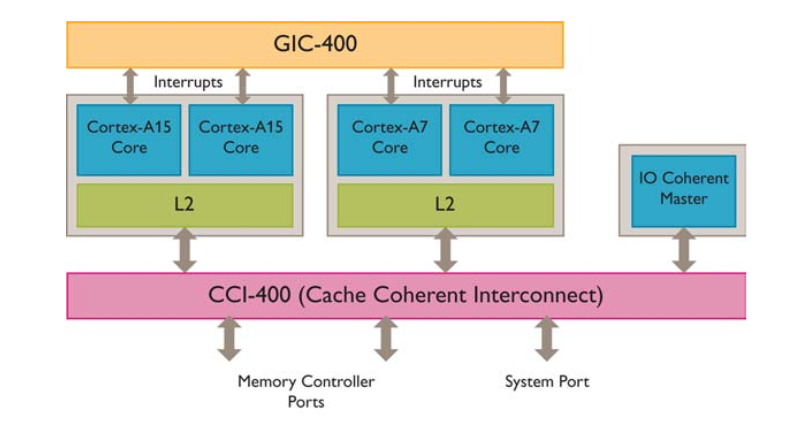
\includegraphics[width=1\textwidth]{background/graphics/biglittle.png}
 \caption{Example of a heterogeneous multicore processor proposed by ARM (big.LITTLE)}\label{fig:blarm}
\end{figure}


\section{Dynamic Multicore Processors}

% This section explains what a dynamic multicore is

In both CMPs and HCMPs, once the chip is fabricated the design cannot be modified, meaning that many of the trade-offs between power, performance and area cannot be changed after production.
Dynamic Multicore Processors (DMPs) attempt to bridge the gap between the two previous designs by allowing the execution substrate to adapt dynamically at runtime.
Mitall's survey ~\cite{MittalSurv2016} defines three types of modifiable resources: the core count~\cite{ipek2007CoreFusion}, number of resources that each core has~\cite{Homayoun3DPooling2012} and microarchitectural features~\cite{fallinhetblock2014,BauerRSE08,tavanaElastic}.
In this thesis I focus on DMPs that modify the core count.

Here, a DMP is composed of a group of homogeneous cores with a reconfigurable fabric.
The advantage of DMPs over the traditional CMP is the ability to reconfigure the processor to better match the tasks at hand.
For example, large sequential sections of code with high Instruction Level Parallelism (ILP) can be accelerated on a set of fused cores that mimic a wide superscalar processor.
On a parallel workload the DMP can be reconfigured by splitting the fused cores to match the Thread Level Parallelism (TLP).

\begin{figure}[t]
    \centering
    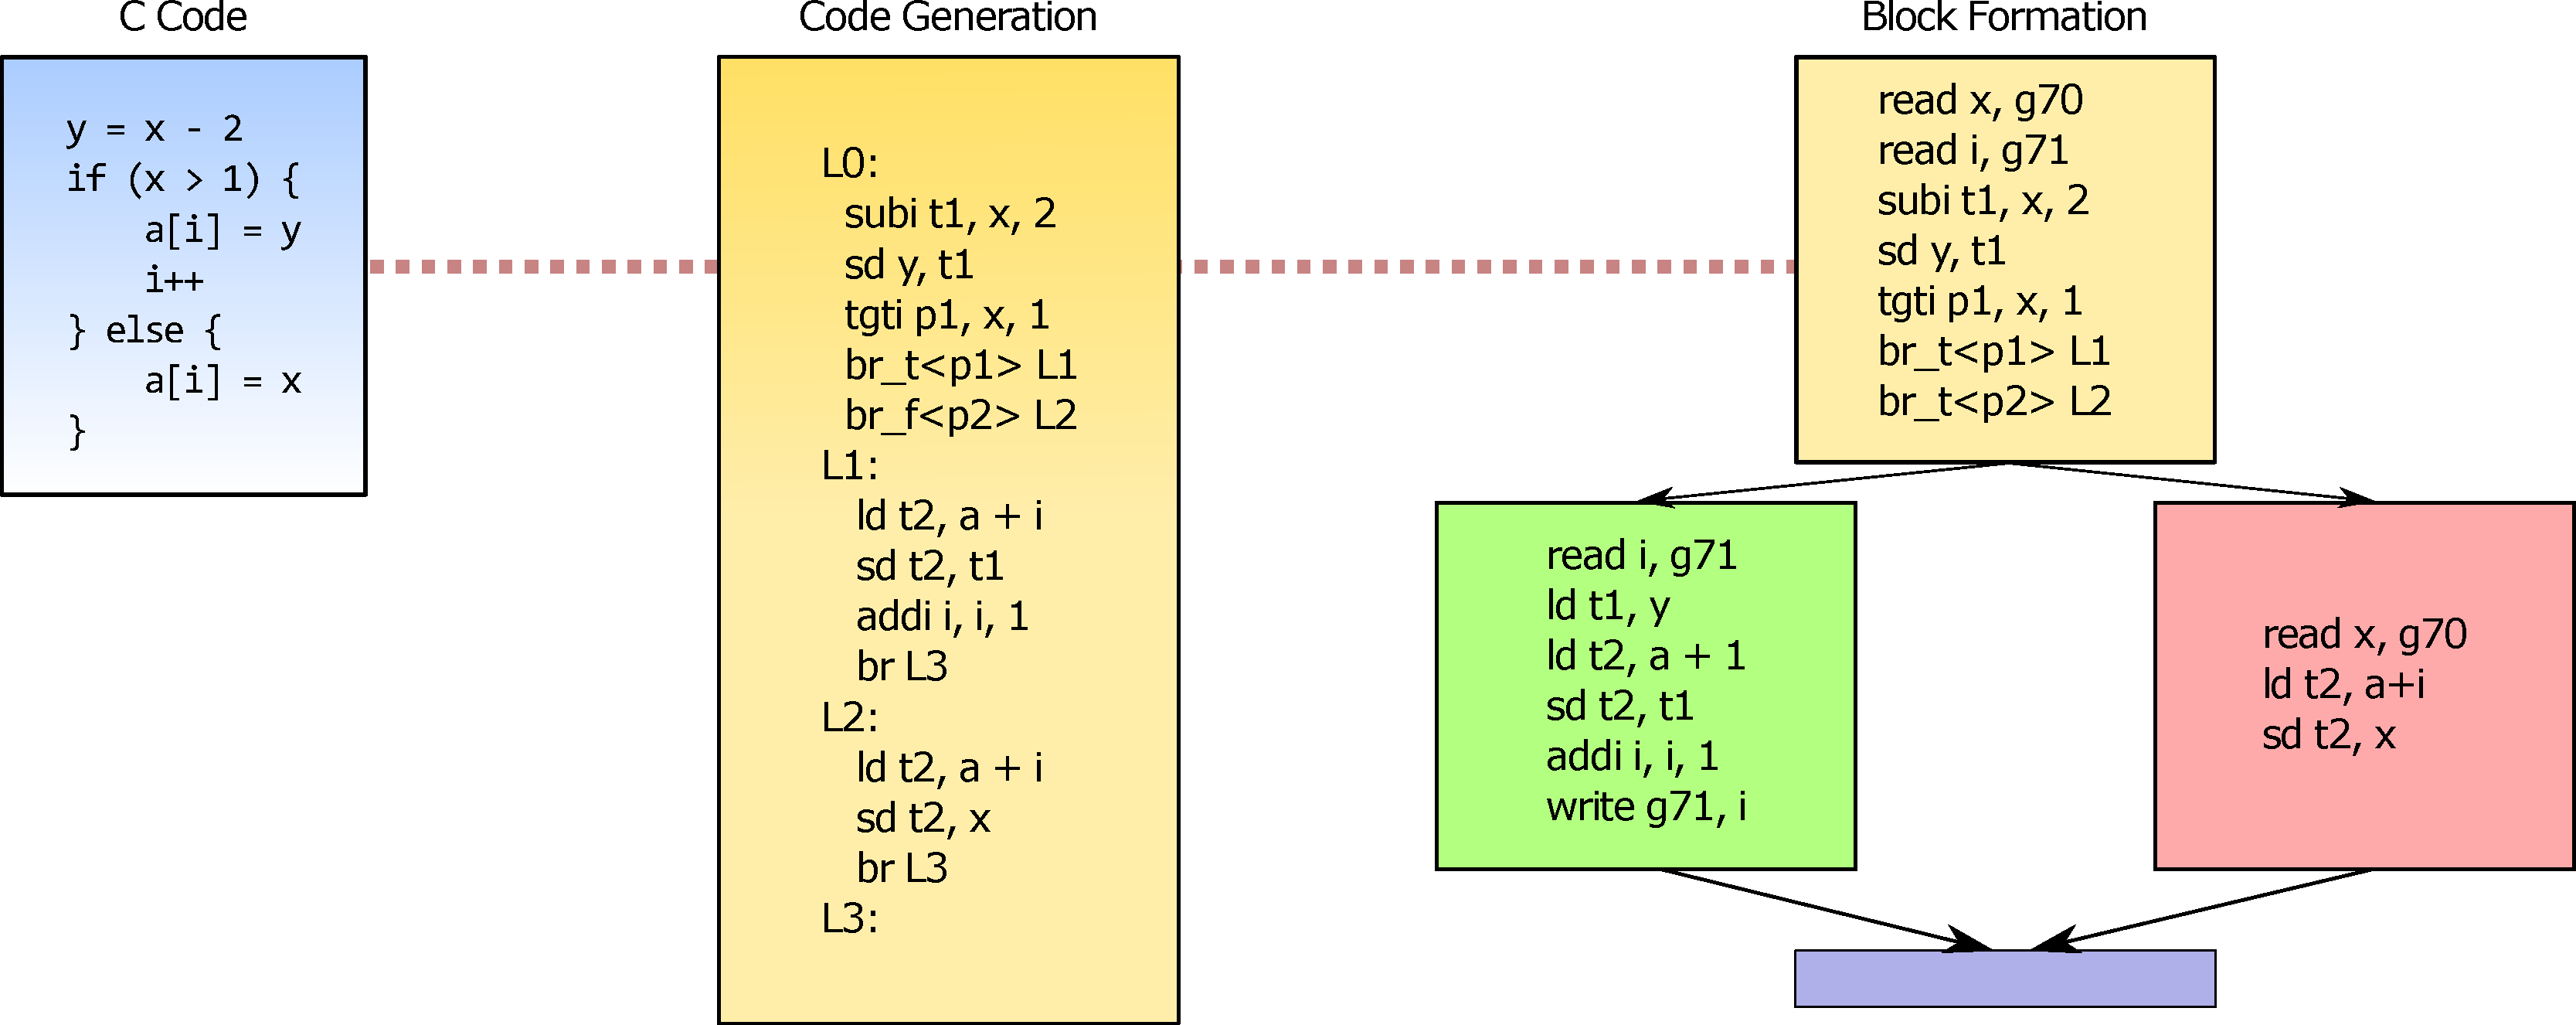
\includegraphics[width=1\textwidth]{background/graphics/EDGE_3.pdf}
    \caption{High-level view of the EDGE ISA flow.}
    \label{fig:EdgeHigh}
\end{figure}
\section{EDGE ISA} We assume a DMP similar to TFlex~\cite{kim2007tflex} using an Explicit Data Graph Execution~\cite{burger04edge} (EDGE) instruction set architecture (ISA).
EDGE ISAs encode dependencies between instructions at the ISA level.
Code is organised as blocks of instructions where all instruction communication is local to the block~\cite{smith2006edge}.
Each block has a single entry point but may have multiple exits.
This enables the architecture to dispatch blocks speculatively, with low overhead~\cite{putnam2010e2,kim2007tflex}, therefore, increasing exploitation of ILP.

\subsection{Core Fusion}
 \begin{figure}[t]
 \center
 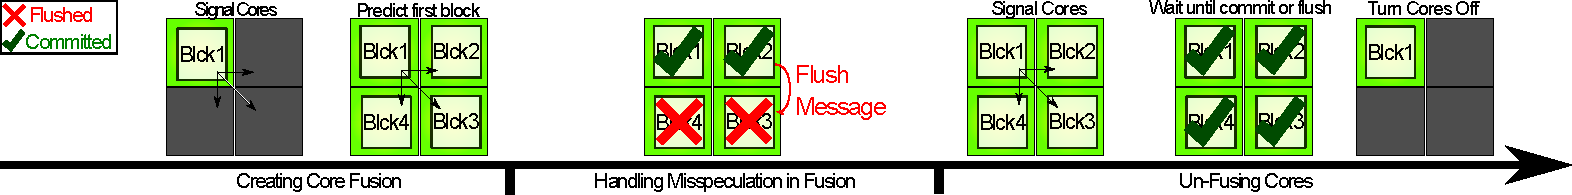
\includegraphics[width=1\textwidth]{cases-paper/graphics/background/proc_test.pdf}
 \caption{Core Fusion Mechanisms for our EDGE-based architecture.}\label{fig:dmp}
 \end{figure}
 
Core Fusion is achieved by fusing a set of \textit{physical} cores to create larger \textit{logical} cores.
This does not modify the physical structure of the chip, instead it provides a unified view of a group of physical cores to the software.
For example, fusing two cores generates a logical core with twice the amount of execution units, register files and L1 cache.
Fusion is a dynamic modification and may occur during the execution of a program to better fit the workload.
Unlike traditional CMPs, fused cores will operate on the same thread and attempt to extract Instruction Level Parallelism (ILP) rather than Thread Level Parallelism (TLP)~\cite{micolet2016dmpstream,pricopi2012bahurupi}.
Figure~\ref{fig:dmp} shows the different stages and mechanisms of core fusion for a four core system.
When creating a new core fusion a master core informs all other cores about the fusion and sends the predicted next block address to the next available fused core.
When a core mispredicts a branch in a fusion, it informs the other cores which flush any younger blocks.
When un-fusing, the master core informs the other cores, which then commit or flush their blocks and power down while the master core continues to fetch and execute blocks from the thread.
The extra hardware required to support dynamic reconfiguration is very minimal~\cite{kim2007tflex} since most of the machinery already in place can be reused such as the cache coherence protocol when fusing and un-fusing the cores.
We discuss this in further detail in Section~\ref{sec:setup}.

%\begin{figure}[t]
%    \centering
%    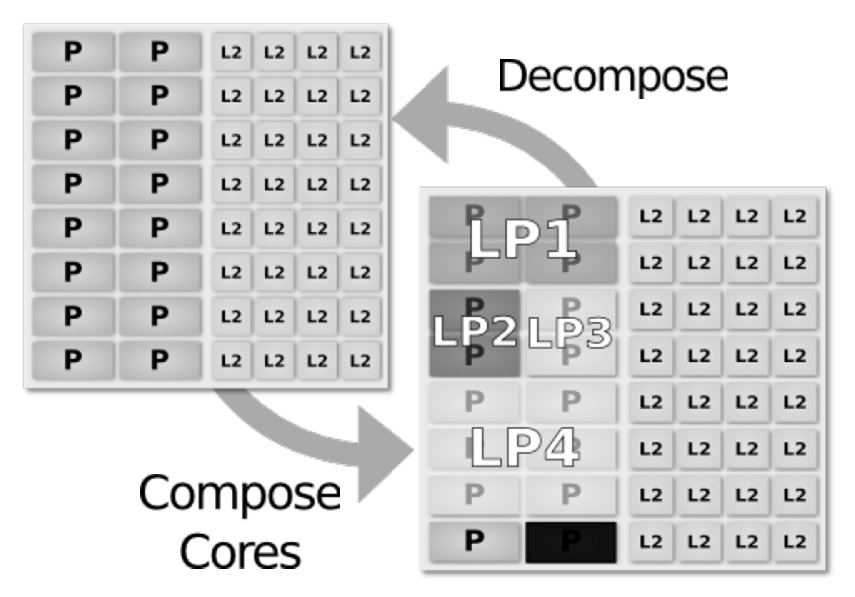
\includegraphics[width=.7\textwidth]{streamit-paper/graphics/dmcgraph.pdf}
%    \caption{High-level view of a dynamic multicore processor considered in this paper.}
%    \label{fig:dynmulticore}
%\end{figure}

%Explain the figure
%In this paper we consider a dynamic multicore processor which allows cores to compose their execution resources, register files and private L1 caches to create logical processors to accelerate a single thread.
%Figure~\ref{fig:dynmulticore} shows a high-level view of the architecture and the two possible states: composed and decomposed.
%The composed state represents a set of physical cores fused to create a larger logical core.
%Multiple sets of cores can be fused to create logical cores of different sizes.
%In Figure~\ref{fig:dynmulticore} for example, LP1 is composed of four physical cores whereas LP2 is composed of two.
%At runtime, physical cores may be decomposed from a logical processor to remove them from the core composition.

\section{Streaming Programming Languages}

% % This section should explain what steaming programming is (remove all the details about each language)
% General purpose programming languages often propose very little support for programs that handle with a continuous flow of data.
% This results in having to design a set of complicated for loops to manage the streams of data.
% Having to deal with different rates of incoming and outcoming data also increases the complexity of writing these applications using a standard language.

Streaming programming languages are a branch of dataflow programming that focus on applications that deal with a constant stream of data.
These applications, such as audio or video decoding can be commonly found in mobile devices.
Unlike conventional programming languages such as C++, these languages abstract the concept of incoming and outgoing data to permit the programmer to focus on how the data should be treated.
Programs are described as directed graphs where nodes are functions and their edges represent their input and output streams. 
These languages offer primitives to describe such a graph~\cite{theis2002streamit} which expose parallelizable and serial sections of the application directly to the compiler. 
Rates of incoming and outcoming data can also be defined to facilitate load balancing optimizations~\cite{chen2005rawstream}.

Features of streaming programming languages make them an ideal language for targeting multicore processors.
The explicit data communication between the different tasks in the program, the ability to estimate the amount of work performed in each task and information about data rates between tasks allows the compiler to easily generate a multi-threaded application that can run on a dynamic multicore processor.
However, the main challenge consists of deciding how to map the different tasks onto threads and how to allocate the right amount of resources to maximize performance.



\section{Experimental Setup}
This section describes the setup used throughout this chapter to conduct the design space exploration.
It starts by presenting the overall workflow and then explores briefly some of the features of the benchmarks.
Finally the section explains how the number of design points used throughout the exploration were determined.

\begin{figure}[t]
    \centering
    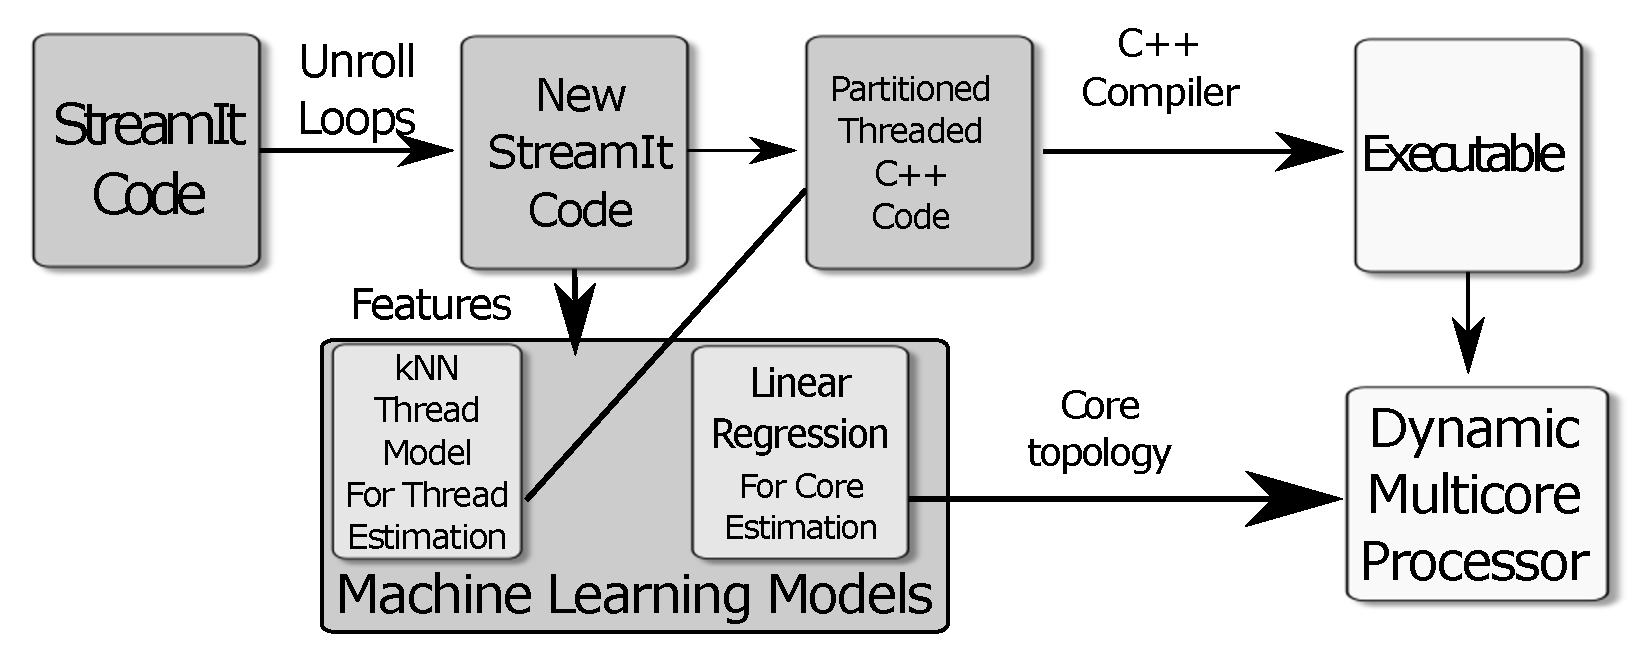
\includegraphics[width=1\textwidth]{streamit-paper/graphics/explanation3.pdf}
    \caption{Description of the workflow.
    Two distinct machine-learning models are used to predict the optimal thread partitioning and core composition based on static code features.}
    \label{fig:overview}
\end{figure}

\subsection{Overview}

\begin{figure}[t]
    \centering
    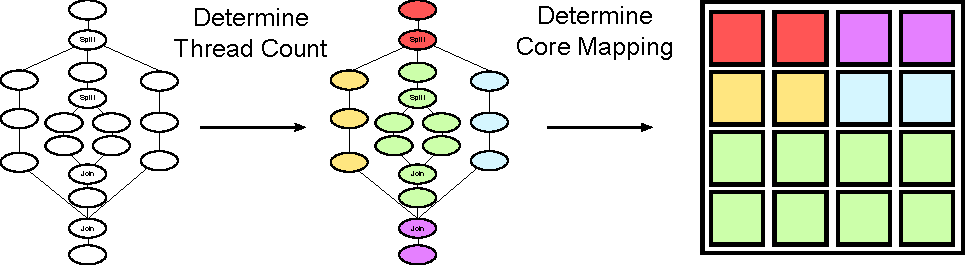
\includegraphics[width=1\textwidth]{streamit-paper/graphics/examplestrem.pdf}
    \caption{Example of a StreamIt program being partitioned into threads (represented by the different colours) followed by assigning cores to each thread.}
    \label{fig:examplestream}
\end{figure}

Figure~\ref{fig:overview} presents the workflow of the system used in this chapter and Figure~\ref{fig:examplestream} illustrates the workflow on a synthetic StreamIt graph.
First, the source-to-source StreamIt compiler is used to unroll loops as this is often beneficial when cores are composed as will be seen later in Section~\ref{sec:streamit:dse}.
Then, static code features such as the program's graph structure are extracted from the StreamIt code through the StreamIt source-to-source compiler.
These features are used as an input to the first machine-learning model that determines how many threads will be required based on an estimate of Thread Level Parallelism (TLP) found in the program.
This information is used to partition the program into threads which is done by the StreamIt compiler which produces a C++ program using pthreads.
This is exemplified in Figure~\ref{fig:examplestream}, the colours filling in the nodes represent the threads each node has been assign to.
This C++ program is then compiled using the compiler for EDGE described in Chapter~\ref{chp:setup} Section~\ref{chp:setup:comp}.

Then, a second machine-learning model is deployed which also analyses static code features extracted from the SteamIt code, once again provided by the source-to-source compiler.
This model decides on the number of cores each thread will have.
This is achieved by estimating the amount of Instruction Level Parallelism (ILP) that can be possibly extracted in each thread and by determining how many physical cores should be fused for that thread.
Finally, the processor is reconfigured to compose the requested resources ahead of time and execute the partitioned program.
For example in Figure~\ref{fig:examplestream}, once the graph is coloured, the machine learning model estimates the potential ILP in each group and assigns a number of cores each thread will execute on.

\subsection{Design Space}

The benchmarks used throughout this chapter are shown in Chapter~\ref{chp:setup} Section~\ref{chp:setup:streamit}.
These applications represent a variety of embedded applications and kernels, from digital signal processing to a matrix-multiplication kernel or band pass filters.
Table~\ref{tab:instancefilt} shows the number of filter instances and SplitJoins for each of the benchmarks.
As a refresher from Chapter~\ref{chp:Background} Section~\ref{chp:bckg:streamit}, SplitJoin filters are functions which distribute and collect data from parallel filters.
The applications feature a different number of SplitJoins which determine the task-level parallelism.
This is to include a variety of situations to test the flexibility of the dynamic multicore processor.
Whilst SplitJoins often facilitate the decision of how to partition the programs into threads, they are not the only way to exploit thread level parallelism.
The applications which do not feature SplitJoins can still be split into threads and will operate in a pipelined fashion~\cite{theis2002streamit}.
For each benchmark the default inputs provided in the repository~\cite{streamitrepo} are used and the default iteration count is set to 10. 

\begin{table}[t]
% The FFT need are variable
  \small
 \begin{tabular} { | l | l | l | l | l | l | }
 \hline
 \cellcolor[gray]{0.7}Type  & \cellcolor[gray]{0.7}Audiobeam&  \cellcolor[gray]{0.7} Beamformer& \cellcolor[gray]{0.7}Bitonic-Sort  &  \cellcolor[gray]{0.7} BubbleSort &  \cellcolor[gray]{0.7}  CFAR\\ \hline
  Filter Instances & 18 & 56 & 82 & 18 & 3 \\ \hline
	\# of SplitJoins &	1 & 2 & 44 & 0 & 0 \\ \hline

 \cellcolor[gray]{0.7}Type  & \cellcolor[gray]{0.7}ChannelVocoder &  \cellcolor[gray]{0.7} FFT&  \cellcolor[gray]{0.7}FFT3 &  \cellcolor[gray]{0.7} FFT6&  \cellcolor[gray]{0.7}FilterBank \\ \hline
  Filter Instances & 53 & 20 & 185 & 99 & 67 \\ \hline 
   \# of SplitJoins &	 1 & 12 & 44 & 96 & 9 \\ \hline 

   \cellcolor[gray]{0.7}Type& \cellcolor[gray]{0.7}FIR &  \cellcolor[gray]{0.7} FMRadio &  \cellcolor[gray]{0.7} InsertionSort &  \cellcolor[gray]{0.7} Matmul-Block &  \cellcolor[gray]{0.7} RadixSort\\ \hline
  Filter Instances& 131 & 29 & 6 & 4 & 13 \\ \hline
  \# of SplitJoins&    0 & 7 & 0 & 7 & 0 \\ \hline

 \end{tabular}
  \caption{Number of filter instances and SplitJoin filters present in each benchmark.}\label{tab:instancefilt}
\end{table}

%\begin{table}[t]
% The FFT need are variable
 % \small
 %\begin{tabular} { | l | l | l | l | l | }
 %\hline
 %  \cellcolor[gray]{0.7}Audiobeam&  \cellcolor[gray]{0.7} Beamformer& \cellcolor[gray]{0.7}Bitonic-Sort  &  \cellcolor[gray]{0.7} BubbleSort &  \cellcolor[gray]{0.7}  CFAR\\ \hline
 % 1 & 2 & 44 & 0 & 0 \\ \hline
 %  \cellcolor[gray]{0.7}ChannelVocoder &  \cellcolor[gray]{0.7} FFT&  \cellcolor[gray]{0.7}FFT3 &  \cellcolor[gray]{0.7} FFT6&  \cellcolor[gray]{0.7}FilterBank \\ \hline
 % 1 & 12 & 44 & 96 & 9 \\ \hline 
 %  \cellcolor[gray]{0.7}FIR &  \cellcolor[gray]{0.7} FMRadio &  \cellcolor[gray]{0.7} InsertionSort &  \cellcolor[gray]{0.7} Matmul-Block &  \cellcolor[gray]{0.7} RadixSort\\ \hline
 % 0 & 7 & 0 & 7 & 0 \\ \hline
% \end{tabular}
%  \caption{Number of split joins present in each benchmark.}\label{tab:splitjoin}
%\end{table}

\begin{table}[t]
\centering
\begin{tabular} { p{5.2cm}  p{1.8cm} }
      \toprule
      \textbf{Parameter} & \textbf{Values} \\ \midrule
      \# of cores in the processor & 16 \\
      \# threads per application & 1 -- 15 \\
      \# cores per thread & 1 -- 15 \\ \midrule
      \# sampled core compositions & 100 \\ 
      \# our sampled space & 1316 \\
      \# total sample space & 32767 \\ \bottomrule
    \end{tabular}
  \caption{Design space considered per application.}
  \label{tab:space}
\end{table}

The parameters and size of the space are given in Table~\ref{tab:space}.
In this study the 16 core DMP defined in Chapter~\ref{chp:setup} Section~\ref{chp:setup:conf} is used.
Having 16 cores allows for a larger variety of configurations, this also represents a processor similar to a tiled embedded system such as Tilera or Raw.
All cores in the DMP are utilised; Core 0 is assigned to the main thread and for runtime management.
This leaves 15 cores available for each application.
Each core is restricted to running only a single thread, as no context switching is supported, which leads to a possible number of threads between 1 and 15.
The core-composition is not used on the master core, leaving 15 physical cores to be distributed to each of the worker threads.
Cores can be composed together to form a composition with up to 15 physical cores, making the total number of cores assigned to a thread between 1 and 15.
Of course, not all cores have to be assigned to a thread, in this case all remaining cores that aren't in a composition or a thread are turned off.
Overall, this leads to a total space size of 32,767 unique combination per benchmark as previously described in Section~\ref{sec:motivation}.

\subsection{Sample Space}

Given a partition, any benchmark that can be split into 15 threads requires 32,767 executions to cover the entire space.
Running the exhaustive exploration of the space for a benchmark requires approximately a week of simulation on a 572+ node supercomputer.
For this reason, a sample of 1,316 random points from the entire space is utilised.
This roughly corresponds to 100 core compositions for each number of threads; the actual number, 1,316 is smaller than 1,500 since for low and high thread counts there are less than 100 possible different core composition.
For example, a single thread can have only up to 15 different core-compositions (1 through 15) whilst 15 threads can only have a single core given to each thread.
\bench{InsertionSort} is the only exception since it can at most only be split into 5 threads leading to 415 sample points.
Overall, the space exploration required one week of simulation on the supercomputer~\cite{ecdf}.

\begin{figure}[t]
  \centering
    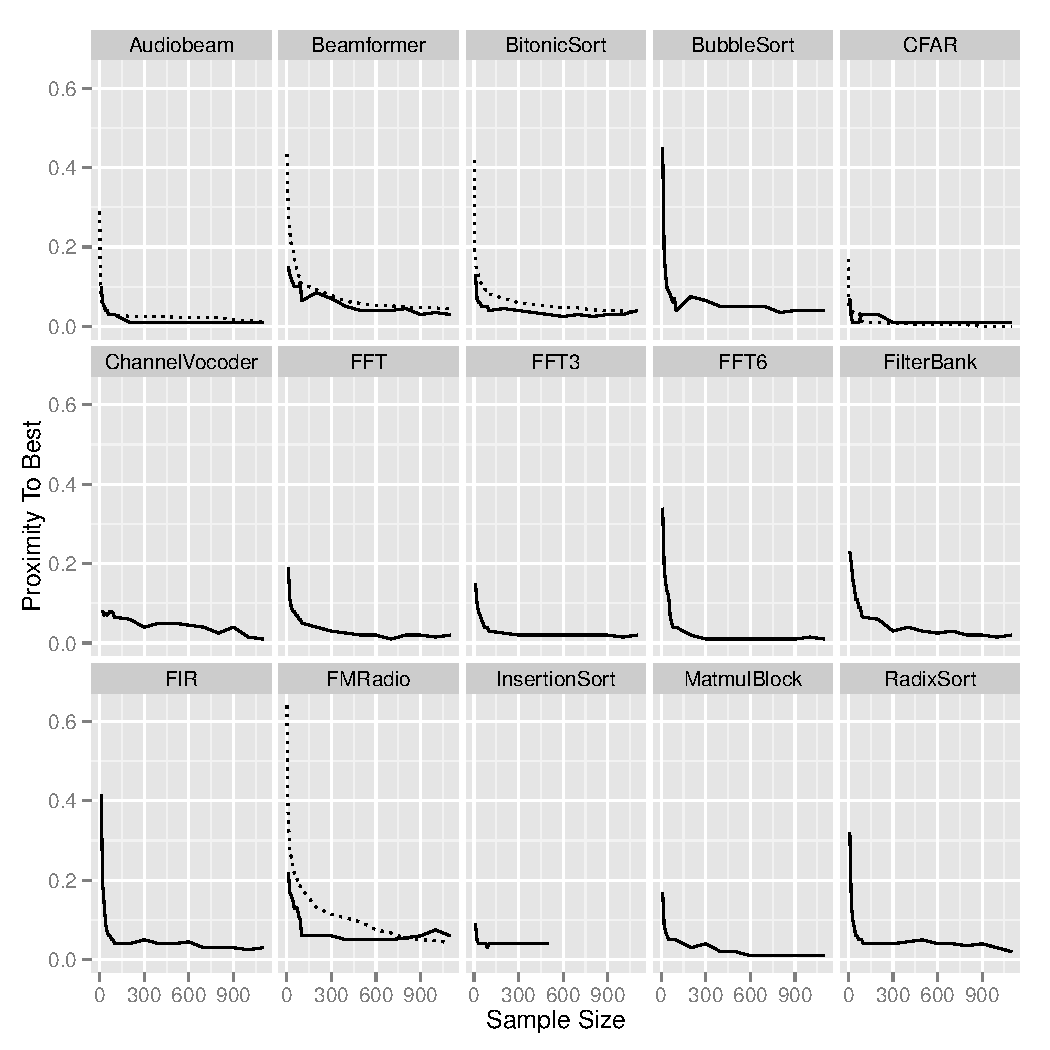
\includegraphics[width=1\textwidth]{streamit-paper/graphics/ESCProx.pdf}
    \caption{Statistical (plain line) and actual proximity (dotted line, this is only done for 5 benchmarks) to best performance using a subset of the sample space.}\label{fig:prox}
\end{figure}

%Define stopping criterion?
To gain confidence that the best configuration from the sample space is indeed close to the real best in the entire space, a statistical model based on the Early Stopping Criterion defined in~\cite{vuduc2003AutomaticPerf} is deployed.
This statistical model estimates, given a sample of the total space, if the best observed performance of that sample space is within a percentage of the statistical best performance, a more detailed explanation can be found in Chapter~\ref{chp:Background} Section~\ref{sec:esc}.
The results demonstrate that the sample space selected is representative of the whole space.

Figure~\ref{fig:prox} shows, for each of the benchmarks, the proximity to the statistical best when increasing the sub-sample space given a maximal uncertainty of 5\%  (\ie minimum 95\% confidence).
As can be seen by the plain line, the model shows that the best sample point is actually within 5\% (0.05 proximity) of the best for all the benchmark.
The proximity is measured by taking the best currently observed point and comparing it to the latest discovered point.
To further prove that the statistical model based on the Stopping Criterion is indeed accurate, an exhaustive exploration of five benchmarks is conducted.
The dotted line in figure~\ref{fig:prox} shows the actual proximity to the best for \bench{Audiobeam}, \bench{Beamformer}, \bench{BitonicSort}, \bench{CFAR} and \bench{FMRadio}.
As can be seen after 1316 samples, the achieved performance is actually very similar to the one predicted by the statistical model, hence confirming prior work~\cite{vuduc2003AutomaticPerf}.
To summarise, it can be concluded that the best point found in the sample space of 1,316 points is at least within 5\% of the real best in the exhaustive space with 95\% confidence.

\subsection{Synthetic Benchmarks}

\begin{table}[t]
% The FFT need are variable
  \small
 \begin{tabular} { | l | l | l | }
 \hline
 & Av. Number of SplitJoins & Average Number of Filter Instances \\ \hline
 Selected Benchmarks & 14 & 52 \\ \hline 
 Synthetic & 22 & 64 \\ \hline
 \end{tabular}
 \caption{Data on the synthetic benchmarks compared to the selected benchmarks}~\label{tab:synthvsreal}
 \end{table}

One of the difficulties of building a machine learning based model for StreamIt is the lack of a large amount benchmarks available~\cite{wang2013partitionstreamit}.
To overcome this problem generating synthetic benchmarks can be a solution~\cite{cumminsopencl2017}.
Thus synthetic StreamIt benchmarks are generated and statistics are gathered from them in a similar style as in~\cite{wang2013partitionstreamit}.
In this chapter, the synthetic benchmarks are used to build a model for predicting the number of threads, which will be described later in section~\ref{sec:ml}

%Cite repository
To ensure that the synthetic benchmarks are representative of realistic benchmarks they are created using filters from a set of example StreamIt programs found in the example directory in the repository.
30 different possible filters with different incoming and outgoing rates and different inputs and outputs types are used to increase the variety of the dataset.
To ensure that the synthetic benchmarks are similar to real benchmarks, the total number of filters and split joins are within the average of the realistic benchmarks.
Table~\ref{tab:synthvsreal} gives the average number of SplitJoins and filter instances for the synthetic benchmarks vs the real benchmarks used in this chapter.
As can be seen, the synthetic benchmarks, on average, have more SplitJoins than the real benchmarks; this is due to the fact that a few of the benchmarks presented in the chapter don't have SplitJoins at all which can quickly reduce the average.
%Maybe say a bit more here.
Since these benchmarks are built to be used for predicting the number of threads an application should use, and SplitJoins are explicit declarations of task-level parallelism, having a higher average number of SplitJoins is not detrimental to building the model.


\section{Design Space Exploration}
\newcommand{\novp}{\textit{\textbf{SFNoVP}}}
\newcommand{\vp}{\textit{\textbf{SFVP}}}
\newcommand{\nfnovp}{\textit{\textbf{RRFNoVP}}}
\newcommand{\nfvp}{\textit{\textbf{RRFVP}}}

\newcommand{\optvp}{\textit{\textbf{OptVP}}}
\newcommand{\vt}{\textit{\textbf{VT}}}
\newcommand{\nfvt}{\textit{\textbf{RFVT}}}
\vspace{-1em}

This section explores how a perfect branch and value predictor, paired with the new fetching scheme (RRF), improves the performance of core composition.
To understand how each component contributes to the performance improvements, different configurations were used, they are as follows:
\begin{itemize}
\item Serial fetching scheme with no value prediction (\novp).
\vspace{-1em}
\item Serial fetching scheme with perfect value prediction (\vp).
\vspace{-1em}
\item Round robin fetching scheme with no value prediction (\nfnovp).
\vspace{-1em}
\item Round robin fetching scheme with value prediction (\nfvp).
\end{itemize}

All configurations use perfect branch prediction  to ensure that core composition is always on the correct execution path.
All benchmarks are executed with 16 cores composed as this is the maximum number of cores that can be fused.
No dynamic adaptation is done as Chapter~\ref{chp:cases} showed that the primary advantage of dynamic core composition is energy savings, whereas this chapter focuses on speedup.


\subsection{Analysing the performance of the different configurations}
Figure~\ref{fig:perf_pred} shows the speedup obtained on the SD-VBS benchmarks using the different configurations.
The baseline for this section is 16 cores composed with serial fetch (SF) no value prediction (\novp) and perfect branch prediction.
This baseline is chosen as this chapter is focused on improving the performance of core composition.

First, it is clear that using RRF with value prediction (\nfvp) always results in the best speedup compared to the baseline.
For \bm{Multi\_NCut}, performance is improved by 3x when using \nfvp.
This is a significant speedup, as Chapter~\ref{chp:cases} showed that \bm{Multi\_Ncut} is a difficult benchmark for core composition (1.3x speedup in Chapter~\ref{chp:cases}).
On average, \nfvp{} outperforms the baseline by a factor of 1.88x.

\begin{figure}[t]
    \centering
    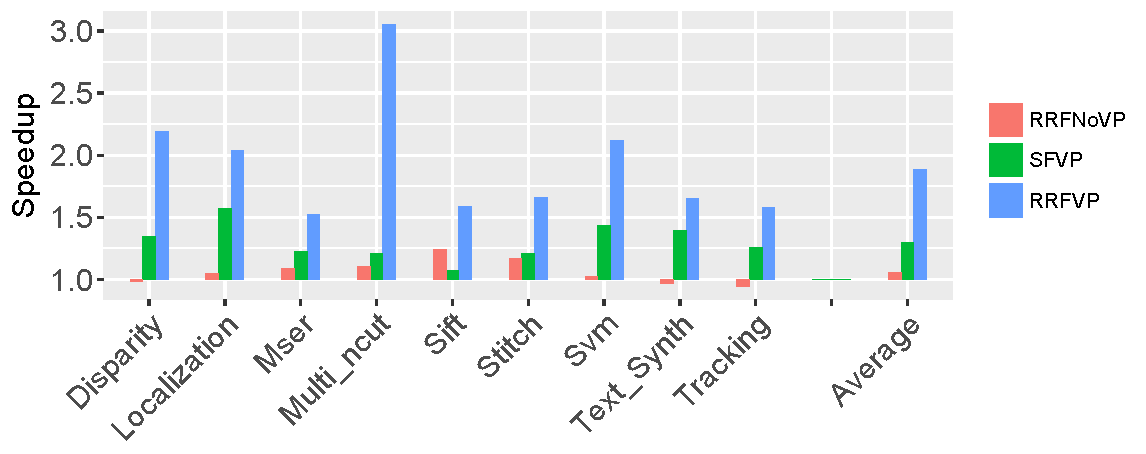
\includegraphics[width=1\textwidth]{chapter3/graphics/tempres4.pdf}
    \caption{Comparing the performance of serial fetch to round robin fetch, with and without perfect value prediction. Higher is better}
    \label{fig:perf_pred}
\end{figure}

\subsubsection{Performance without value prediction}
The results in Figure~\ref{fig:perf_pred} show that without value prediction the performance improvements brought by RRF on its own are low, or in fact detrimental to performance.
For example, \bm{Multi\_NCut} only has a 1.10x speedup when using the \nfnovp{} configuration, compared to the 3x of \nfvp{}.
This is due to the fact that whilst more blocks are now spread across cores, the register dependencies between blocks limit the performance of the composition. 
In fact, the more even distribution is the reason why some benchmarks perform worse: \bm{Disparity}, \bm{Texture\_Synthesis} and \bm{Tracking} see a slight performance decrease.
The even distribution of blocks amongst cores increases the stress on the network on chip (NoC) as more cores will make accesses in parallel.
Without value prediction, RRF suffers due to NoC stress and data dependencies.
%In fact, \vp{} outperforms \nfnovp{} on \bm{Localization}, which shows that register dependencies between blocks can make the new fetching scheme less performant than the currently implemented.

%The performance limitations are caused by blocks that are further down the speculative path that must wait for older blocks to write to the register file.


\subsubsection{Performance with value prediction}
The performance improvements brought by RRF are more apparent when taking value prediction into account.
\nfvp{} has a 54\% performance increase compared to \vp{} (1.88x vs 1.22x).
The difference in performance comes from the fact that with value prediction, blocks can potentially execute faster, and thus a faster fetching scheme is required to keep up.
Since the SF scheme is slower, it is less likely going to benefit from parallel execution.
Even so, \vp{} results in a 1.5x speedup for \bm{Localization} which shows that value prediction is valuable for composition regardless of the scheme.

\begin{figure}[t]
    \centering
    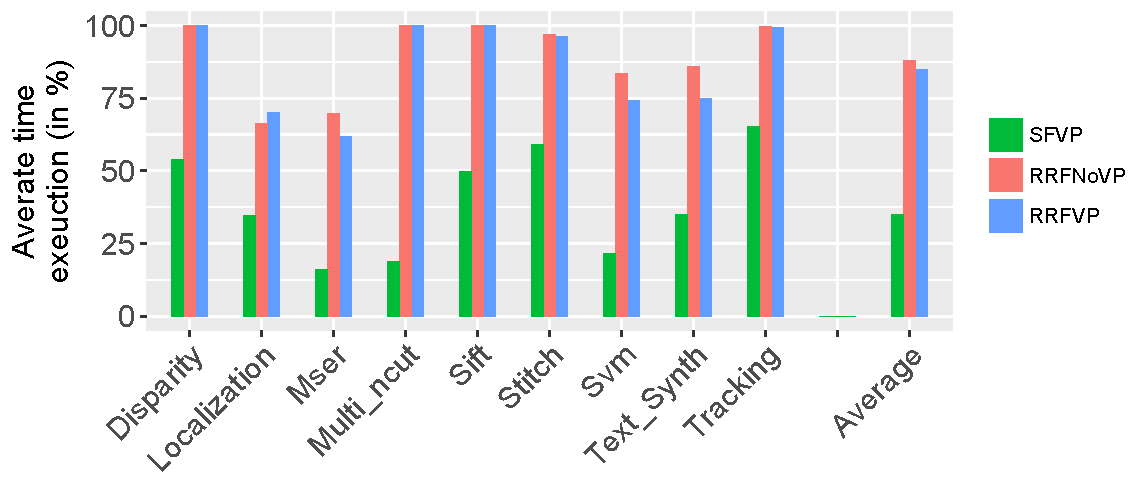
\includegraphics[width=1\textwidth]{chapter3/graphics/perf_av_cycle_exec4.pdf}
    \caption{Average time each core is executing blocks (in \%) for each benchmark, using the different configurations. Higher is better.}
    \label{fig:perf_av_cycle}
	\vspace{1em}
\end{figure}

\paragraph*{Active Cycles}
To better highlight how the SF scheme hinders performance even with value prediction, the percentage of time a core in a composition is actively executing code, for each benchmark, is shown in Figure~\ref{fig:perf_av_cycle}.
For each configuration, the number of cycles each core in a composition has instructions to execute is averaged out and then compared to the total execution time of the application.
When the average active time of a core is close to the total execution time, this means that the composition was efficiently used, as each core had a block to run throughout the program execution.

Figure~\ref{fig:perf_av_cycle} shows that \vp{} often has low active times when using a composition of 16 cores.
This is due to the fact that the SF scheme is slow, and thus, some cores are inactive, waiting to receive a fetch request from another core.
The lower the percentage is, the less likely there are going to be multiple blocks on different cores in flight which in turn means the composition is less efficient and value prediction is less useful.
Since value prediction is aimed at increasing instruction level parallelism (ILP)~\cite{peraisBeBop2015} it is important that cores may fetch blocks quickly in a composition.

%Of course, it is important to note that their LSQs and L1 caches may still be used by other active cores, simply that their execution units are not being used.


With the RRF scheme, the percentage of active time is increased on average by a factor of 2.28x, and is on average 85\%.
This means that during most of the execution of an application, all cores are executing code, and thus greatly increases the chance of improving performance via core composition.
It is interesting to see that \nfvp{} has a lower average time than \nfnovp{} for some benchmarks such as \bm{MSER} and \bm{Texture\_Synthesis}.
Also, whilst RRF aims to evenly distribute blocks amongst the cores, the average core utilisation for \bm{Localization} with the configurations \nfnovp{} and \nfvp{} is of 62\%.
This reduced average time is due to flushes caused by Load-Store-Queue (LSQ) violations, which causes cores to flush their instruction windows, and thus increases the number of times that cores will not be executing code.
Figure~\ref{fig:lsqvio} shows the number of blocks that cause an LSQ violation, normalised by the number of fetched blocks for each of the benchmarks.
Even though the percentage of violations is small, it still has an impact on how efficient the composition is, due to the fact that compositions rely on heavy speculation to obtain any performance improvements.
\begin{figure}[t]
    \centering
    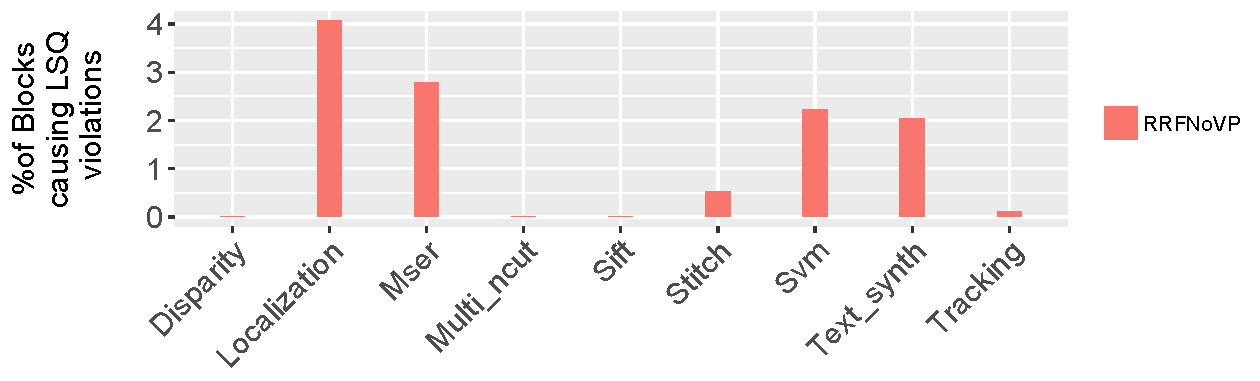
\includegraphics[width=1\textwidth]{chapter3/graphics/lsqViol4.pdf}
    \caption{Number of blocks that cause LSQ violations, normalised by the number of fetched blocks for each of the benchmarks.}
    \label{fig:lsqvio}
	\vspace{1em}
\end{figure}

%A store-set dependency predictor is implemented in the processor~\cite{chrysos1998storesets}, however it is sometimes hard to predict load-store dependencies across multiple blocks, which is why LSQ violations occur.
%Store-set dependency predictors are not discussed in more detail in this chapter, however researching how store-set dependencies could be applied to core-composition is an interesting subject for future work.

\subsection{Round robin fetching scheme bottleneck Analysis}

As seen in the previous section RRF enables better use of the perfect value predictor. 
However, on its own it often does not outperform \novp{}, averaging only a speedup of 1.05x.
This section covers where the bottlenecks of RRF are.%, what potential solutions can be employed, and how that can improve performance overall.

\paragraph*{Block dispatching latency}

RRF improves performance of a core composition by parallelising block fetches.
This is achieved through a round robin fetching scheme, where cores do not fetch blocks sequentially, but rather in strides.
Yet whilst blocks can be fetched out of order they must still be dispatched in order (recall Section~\ref{chp3:sec:fetch}).

\begin{figure}[t]
    \centering
    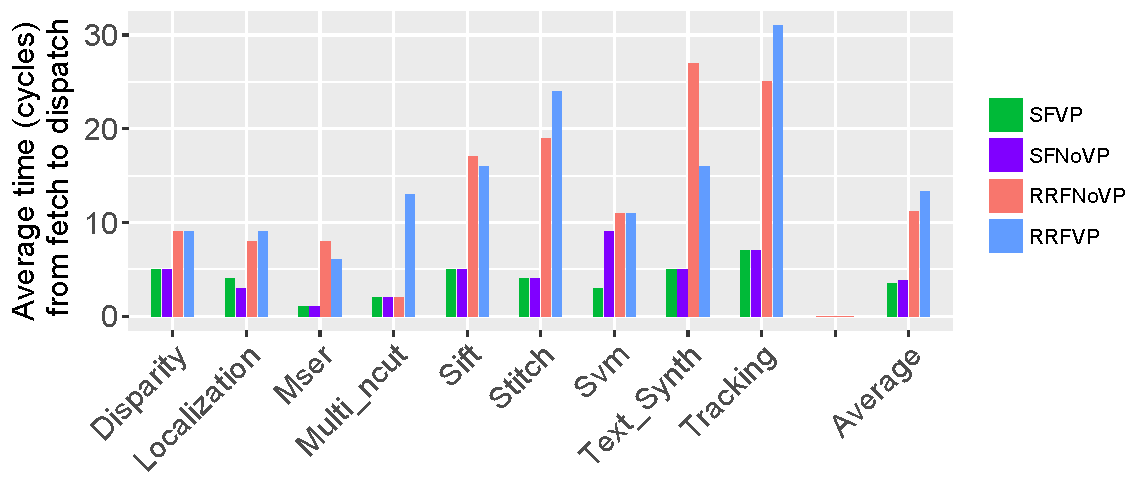
\includegraphics[width=1\textwidth]{chapter3/graphics/avTimeToFetch3.pdf}
    \caption{Average time (in cycles) for block to go from fetched to dispatched using the serial fetching scheme and round robin fetching scheme. Lower is better.}
    \label{fig:av_time}
	\vspace{1em}
\end{figure}

This means that cores may fetch blocks in their window that must wait a certain number of cycles before executing.
To understand how this affects the performance of the new fetching scheme, the average time from a block being fetched, to a block being dispatched is recorded in the simulator.
Comparing the average time between SF and RRF can provide an estimate as to how much performance is potentially lost.

Figure~\ref{fig:av_time} shows the average time for all the SD-VBS benchmarks using the different configurations.
As can be seen, for most benchmarks, RRF's average time is 2x slower than the current.
This is due to the fact that whenever the SF scheme fetches a block, it can immediately dispatched as fetches are serialised.
Surprisingly, \bm{Multi\_NCut} for \nfvp{} has a much longer time between fetching and dispatching a block.
This is due to the fact that \bm{Multi\_NCut} features blocks of only 11 instructions on average and with value prediction blocks are committing faster than on the other configurations.
%Given that a block must access a shared counter to check if it can dispatch, and the counter can only be incremented once per cycle (atomic increment), this shared resource is causing the long fetch to dispatch latency.
Given that only one block can be dispatched per cycle, this is causing the long fetch to dispatch latency.
Even with the extra latency, RRF still ensures that every core is full, cores must now only wait for their blocks to be dispatched, rather than having for a fetch request.

\begin{figure}[t]
    \centering
    
\includegraphics[width=1\textwidth]{chapter3/graphics/fetch_ex.pdf}
    \caption{Two core composition where cores fetch blocks of varying size. Green blocks represent blocks that can be dispatched, whilst the red blocks cannot.}
    \label{fig:var_ex}
    \centering
    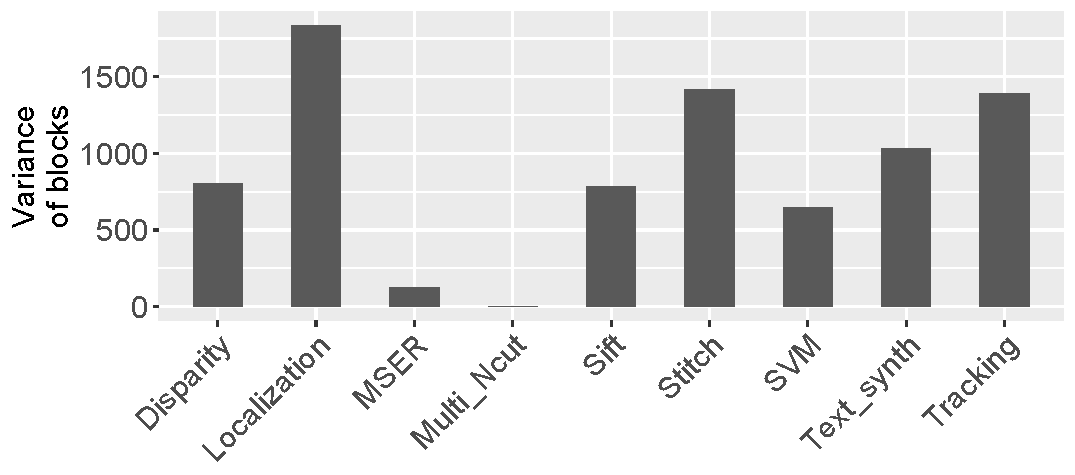
\includegraphics[width=1\textwidth]{chapter3/graphics/variance.pdf}
    \caption{Standard deviation of block sizes per benchmark.}
    \label{fig:variance}
	\vspace{1em}
\end{figure}
\paragraph*{Block size variance}
Another issue that can arise when fetching with a fixed stride is that if cores are fetching blocks of different sizes this may increase the fetch to dispatch latency.
For example, in the two core composition seen in Figure~\ref{fig:var_ex} the second core fetches Block 2 that is 128 instructions.
If Block 2 were smaller, Core 2 could fetch and dispatch blocks 4 and 6.
However, since Block 2 occupies the whole instruction window, Core 2 will have to wait for block 2 to commit before doing so.
Thus blocks 5 and 7 cannot be dispatched on Core 1 before block 2 has finished executing.

Figure~\ref{fig:variance} shows the variance of block sizes in the SD-VBS benchmarks.
This was obtained by counting the different block sizes each benchmark fetched, and grouping them into 4 distinct buckets: blocks that occupy 1, 2, 3 or 4 lanes in the window.
The Figure shows that the benchmark \bm{Multi\_NCut} features a very low variance; which is why RRF has a similar fetch to dispatch latency as SF without value prediction.

%The issue of variance is not only specific to RRF, as SF will also suffer from this issue as well.
%The difference is that with SF, Core 1 would not fetch blocks 3, 5 and 7, instead it would wait for Core 2 to commit its block and submit a fetch request.
%Of course, variance only partially provides an insight as to why core composition may be less efficient; as it does not take into account data dependencies between blocks.
%Also, the variance does not take into account that blocks of different sizes may belong to different phases.
%Nevertheless, it is an important factor to take into consideration.
%. Blocks are grouped up in buckets (occupy 1, 2, 3 or 4 segments).


%Explain how different blcok sizes may mess up the new fetching scheme

\subsubsection{Summary}

This section shows that a perfect branch predictor, paired with perfect value prediction and the round robin fetching scheme can outperform the current configuration by a factor of up to 3x and on average a speedup of 1.87x.%, and can potentially be improved to 2.35x with further modifications to the fetching scheme.
This section also showed that without value prediction RRF only obtains a 1.09x speedup compared to the serial fetching scheme.
This is due to the fact that the benchmarks all display a certain amount of data-dependencies between blocks and that spreading blocks across cores more evenly can put pressure on the NoC; thus reduce the performance improvements of fetching blocks quicker.



\section{Building a model for thread estimation}
% Small intro, re-explain that finding thread/core pairing is complicated and thus ML is a good idea.
As seen in the previous section, selecting the right number of threads and a good combination of cores is difficult.
This difficulty arises from trying to balance between exploiting larger composed cores with block speculation and ILP and between exploiting a larger number of logical cores via TLP.

The problem can be decomposed into two stages; first, determining the right number of threads and then selecting a good core composition.
In this section, two machine-learning models that predict the best thread partitioning and core composition to maximize performance are presented.

\subsection{Synthetic Benchmark Generation}

One of the difficulties of building a machine learning based model for StreamIt is the lack of benchmarks available~\cite{wang2013partitionstreamit}.
Whilst there exists at least 30 realistic applications for StreamIt~\cite{theis2010empericalcharstreamit} this is simply not enough to create a large enough data set.
To overcome this problem generating synthetic benchmarks can be a solution~\cite{cumminsopencl2017}.
Thus synthetic StreamIt benchmarks are generated and statistics are gathered from them in a similar style as in~\cite{wang2013partitionstreamit}.
To ensure that the synthetic benchmarks are representative of realistic benchmarks they are created using filters from a set of micro-kernels found in some StreamIt applications.
30 different possible filters with different incoming and outgoing rates and different inputs and outputs types are used to increase the variety of the dataset.
To ensure that the synthetic benchmarks were similar to real benchmarks, the total number of filters and split joins are within the average of the realistic benchmarks.

For each generated application, 15 different threaded versions are generated.
Each of these versions is ran using a single core per thread and the cycle count is recorded.
This was repeated for 1000 unique randomly generated applications and record the best number of threads each time.

Once the benchmarks have been generated, the next step consists of gathering features for each applications.
In order to build the two machine learning models an initial set of over 50 features are extracted from StreamIt programs.
These features were extracted using pre-existing analytical tools within StreamIt and some counters added specifically for this chapter.
As 50 features may not necessarily contain any valuable information, the features selected for the models were determine through correlation analysis.
%In this section, when discussing correlation we specifically look at which variables correlate with the optimal number of threads.

\subsection{KNN Model}
In this section, variables which correlate with the optimal number of threads are explored.
These features are used by the model to make a prediction about the number of threads to use.
Figure~\ref{fig:corr} shows the 10 variables that correlate the most with determining the optimal thread number.
In StreamIt the term multiplicity references the number of times a filter will have to execute in a time slice when the graph is in a steady state~\cite{gordon2002streamcomp}.

\begin{figure}
  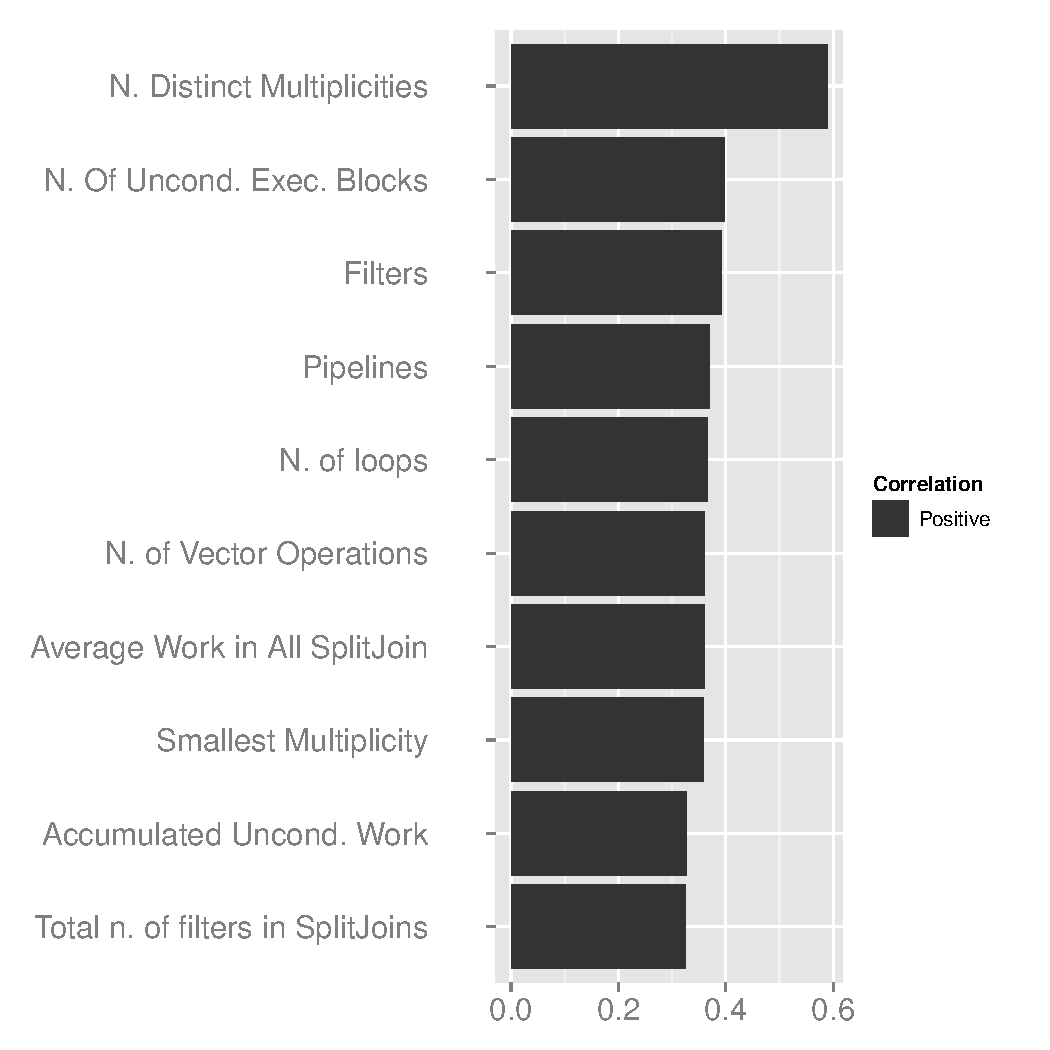
\includegraphics[width=1\textwidth]{streamit-paper/graphics/corrGraph.pdf}
  \caption{The ten highest correlating features with the best number of threads for 1000 synthetic benchmarks.}\label{fig:corr}
\end{figure}
 
\vspace{5em}
The 10 features can be described as followed:
\begin{itemize}
\item Number of Distinct Multiplicities: the variety of different execution rates of filters per time slice.
\item Number of unconditionally executed blocks: amount of operations in a filter that always execute.
\item Filters: number of filters found in the benchmark.
\item Pipelines: number of pipelines found in the benchmark.
\item Number of Loops: amount of loops present in the benchmark.
\item Number of Vector Operations: amount of potential vector operations found in the benchmark.
\item Average Work in all SplitJoins: average amount of operations per SplitJoin.
\item Smallest Multiplicity: The smallest execution rate of a single filter.
\item Accumulated Unconditional Work: Total number of operations in all filters which must be executed.
\item Total Number of filters in SplitJoins: Amount of filters that are found in SplitJoins.
\end{itemize}

According to Figure~\ref{fig:corr} the highest correlating value is Number of Distinct Multiplicitie found in the StreamIt application.
There are very little variables that highly correlate beyond Number of Distinct Multiplicities.
A high number of distinct multiplicities implies that the StreamIt application features an important amount of filters with different execution rates.
This means that certain filters may be local bottlenecks in a Pipeline for example.
When the number of distinct multiplicities is high this requires more threads to group filters with similar multiplicities together.
For example, the benchmark \bench{ChannelVocoder} only has 66\% of its filters sharing the same average multiplicity~\cite{theis2010empericalcharstreamit} of 50, with a minimum multiplicity of 1. 
The benchmark features a single SplitJoin yet when recalling section \ref{sec:streamit:dse}'s Figure~\ref{fig:overviewhist} \bench{ChannelVocoder}'s performance is greatly improved via multi-threading.
The number of threads also depends on certain structural features such as Pipelines, SplitJoins and number of Filters.
Yet, these variables seem to hold less influence on the number of threads a program needs than the different multiplicities found in the graph.
This is most certainly due to the fact that whilst SplitJoins make parallelizable areas more visible, the amount of work contained in each stream of the SplitJoin, especially when this size is small, may actually make parallelizing the program worse due to ratio of communication to computation.
It is also important to understand that a high number of Pipelines implies the use of SplitJoins.
This is due to the fact that a StreamIt application with no SplitJoins will feature only a singe Pipeline, thus a larger number of pipelines implies at least one SplitJoin.\\

A k-Nearest Neighbor (kNN) model is deployed to determine the number of threads to use for an application.
Given a new application, the kNN classifier determines the $k$ closest generated applications.
The distance between the features is measured using the Euclidean for each application.
Once the set of $k$ nearest neighbors is identified, the model simply averages the best number of threads for each of the $k$ nearest neighbors to make a prediction.
The parameter $k$ was determined experimentally using only the generated benchmarks.
A value of $k=7$ was found to lead to the best performance.
The features chosen are the ten variables displayed in Figure~\ref{fig:corr}.

Cross validation is used to determine the efficiency of the model by observing how close a classification is to the measured best thread number.
Using cross validation the model generated in this chapter has a 33\% accuracy of getting the exact best thread number.
The accuracy increases to 57\% when allowing a prediction to be 1 thread away from the best and 67\% when 2 threads away.
On average, having a thread number that is +/- 1 away from the optimal thread count only incurrs a 12\% performance penalty.
For a distance of +/- 2 this increases to 19\%.
This penalty was measured by comparing the performances of the synethtic benchmarks using only multithreading.




\subsection{Predicting the size of a core composition}
In Section~\ref{sec:streamit:dse}, Figure~\ref{fig:threadtrend} showed the performance of each of the 15 benchmarks when partitioning them into threads with and without core-composition.
In both cases, the number of threads is often similar.
The section also demonstrated that loop unrolling can improve the performance of core composition.

Since core composition is used to improve the performance of a single-working-thread, it is important to take into consideration that partitioning the software into threads facilitates the core estimation per thread.
Without determining a number of threads before predicting the number of cores the core-composition model has no information as to the number of threads or the structure of each thread.
In this situation, the core-composition model would either have to make its own estimates as to the thread count, or make a general prediction for a single-working-thread.
Therefore predicting core-composition comes after predicting the number of threads.

\subsubsection{Gathering Training Data for Core-Composition}
For this section the single-working-threaded version of the StreamIt benchmark are used to determine the optimal number of cores in order to explore all possible core composition sizes.
Some of the multi-threaded versions of benchmarks can be used to add extra data-points to build the model, however not all thread-counts are suitable.
One of the difficulties of adding data-points from the highly threaded versions of an applications is that each thread will only be able to have a very small core-composition.
For example, if the 15 threaded version of a benchmarks is added as data points to the model, then each of the feature vectors for this version would have a single core attributed to it.
This is due to the fact that in the 15 threaded versions of benchmarks each thread can only have a single core due to the number of cores on the DMP.
Yet, these threads could potentially benefit from core-composition, so adding them as data points to the model skews future predictions as the feature vector for each thread would associate the features to use only a single core.
Thus high-threaded versions of applications must be ignored to avoid having incorrect suggestions for core-composition sizes.

For the exploration of core composition, the 15 StreamIt benchmarks explored throughout the design space exploration are used. %explain why.
To increase the amount of data available, multiple versions of the benchmarks using different amounts of unrolling are included in the search space.
Four different levels of unrolling are used in to build the model: 0,4,16 and 64.
To determine the optimal number of cores only the training data that has a performance within 1\% of the best is selected.

\begin{figure}[t]
\centering
  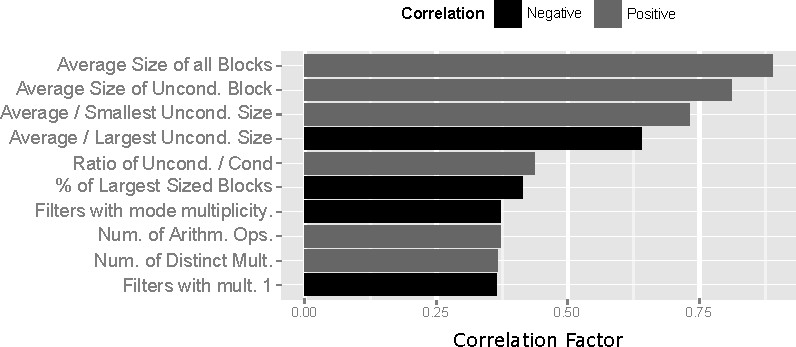
\includegraphics[width=1\textwidth]{streamit-paper/graphics/corrGraph_remix2.pdf}
  \caption{The ten highest correlating features with the optimal number of cores.}\label{fig:corrCore}
\end{figure}


\subsubsection{Correlation Analysis}

Figure~\ref{fig:corrCore} shows the highest correlating features with the optimal number of cores.

The ten features can be described as follows
\begin{itemize}
\item Average Size of All Blocks: Average number of operations per block of code.
\vspace{-1em}
\item Average Size of Unconditional Blocks: Average number of operations per blocks that must execute unconditionally.
\vspace{-1em}
\item Average / Smallest Unconditional Size: The ratio between the average size of a block compared to the smallest size of unconditional blocks.
\vspace{-1em}
\item Average / Largest Unconditional Size: The ratio between the average size of a block compared to the largest size of unconditional blocks.
\vspace{-1em}
\item Ratio of Unconditional Blocks to Conditional Blocks.
\vspace{-1em}
\item Percentage of blocks that have the largest number of operations.
\vspace{-1em}
\item Filters with mode multiplicity: number of filters that have the average mode multiplicity.
\vspace{-1em}
\item Number of arithmetic operations found in the program.
\vspace{-1em}
\item Number of distinct multiplicites found in the program.
\vspace{-1em}
\item Number of filters that have a multiplicity of 1.
\end{itemize}


The features are very different from the ones presented in Figure~\ref{fig:corr} and overall there are features which correlate higher with core-compositions than number of threads.
The highest correlating value, which is the average size of a block, has a correlation factor of 0.88.
It is important to note that the concept of an operation here is at the StreamIt level and not the architectural level.
This is because the machine learning model will get information from the source-level StreamIt translation.
With that in mind, the number of operations will correlate with the number of instructions found at the instruction level.

The second feature is similar to the first but only takes into account blocks that will be executed unconditionally.
Blocks found in loops are excluded for this metric as there is still some form of condition for those blocks to be executed.
The next two features compare the average size of an unconditional block to the largest and smallest unconditional block.
The fifth feature measures the ratio of the number of unconditional blocks to conditional.

Overall the highest correlating features are not features distinct to StreamIt, such as Pipelines or SplitJoins.
This is due to the fact that, from a single-threaded perspective, SplitJoins and Pipelines are less visible in terms of performance.
This is especially true of SplitJoins as they will not be distributing data amongst different threads and, technically, a single-threaded StreamIt program is a long pipeline structure.
It can thus be inferred that the optimal number of cores is independent of the structure of a StreamIt program.
Instead determining the correct core-composition is more dependent on the amount of computation found in each program.

From Figure~\ref{fig:corrCore} the highest correlating features fit naturally under the assumptions that higher core compositions will perform better with larger blocks of operations and thus blocks of instructions.
When blocks are small, a single core can fetch and execute multiple blocks in parallel; up to 4 blocks per core when blocks are smaller than 32 instructions.
Cores in a composition do not fetch blocks independently; instead one of the cores in the composition will start by fetching blocks until all its lanes are used and then submits the following predicted PC to the next core in the composition.
If blocks are small this means that core-compositions will have to predict a high number of blocks to fill up all its cores.
Thus large blocks reduce the number of predictions required to populate all the cores with blocks, reducing the latency of fetching blocks for all cores.
The necessity to correctly predict blocks to ensure that all cores are fully utilised explains why a higher number of unconditionally executed blocks compared to conditional blocks correlates positively with large core compositions.

The importance of size is also apparent as the difference between the largest block size and the average block size negatively correlates with core-composition.
The ratio of unconditional and conditional blocks is considered less important than block size due to branch prediction, however having a larger number of unconditional branches is a natural fit for larger core-compositions as it reduces the dependency on high branch-prediction accuracy.

Other features that are analysed included more fine-grained data such as the types of operations that are found in the blocks of code.
This involved finding ratios of floating point, integer and memory operations.
However, according to the correlation graph in Figure~\ref{fig:corrCore}, the constitution of these blocks of code is not as important as their size or whether they are conditionally executed.

\begin{figure}[t]
  \center
  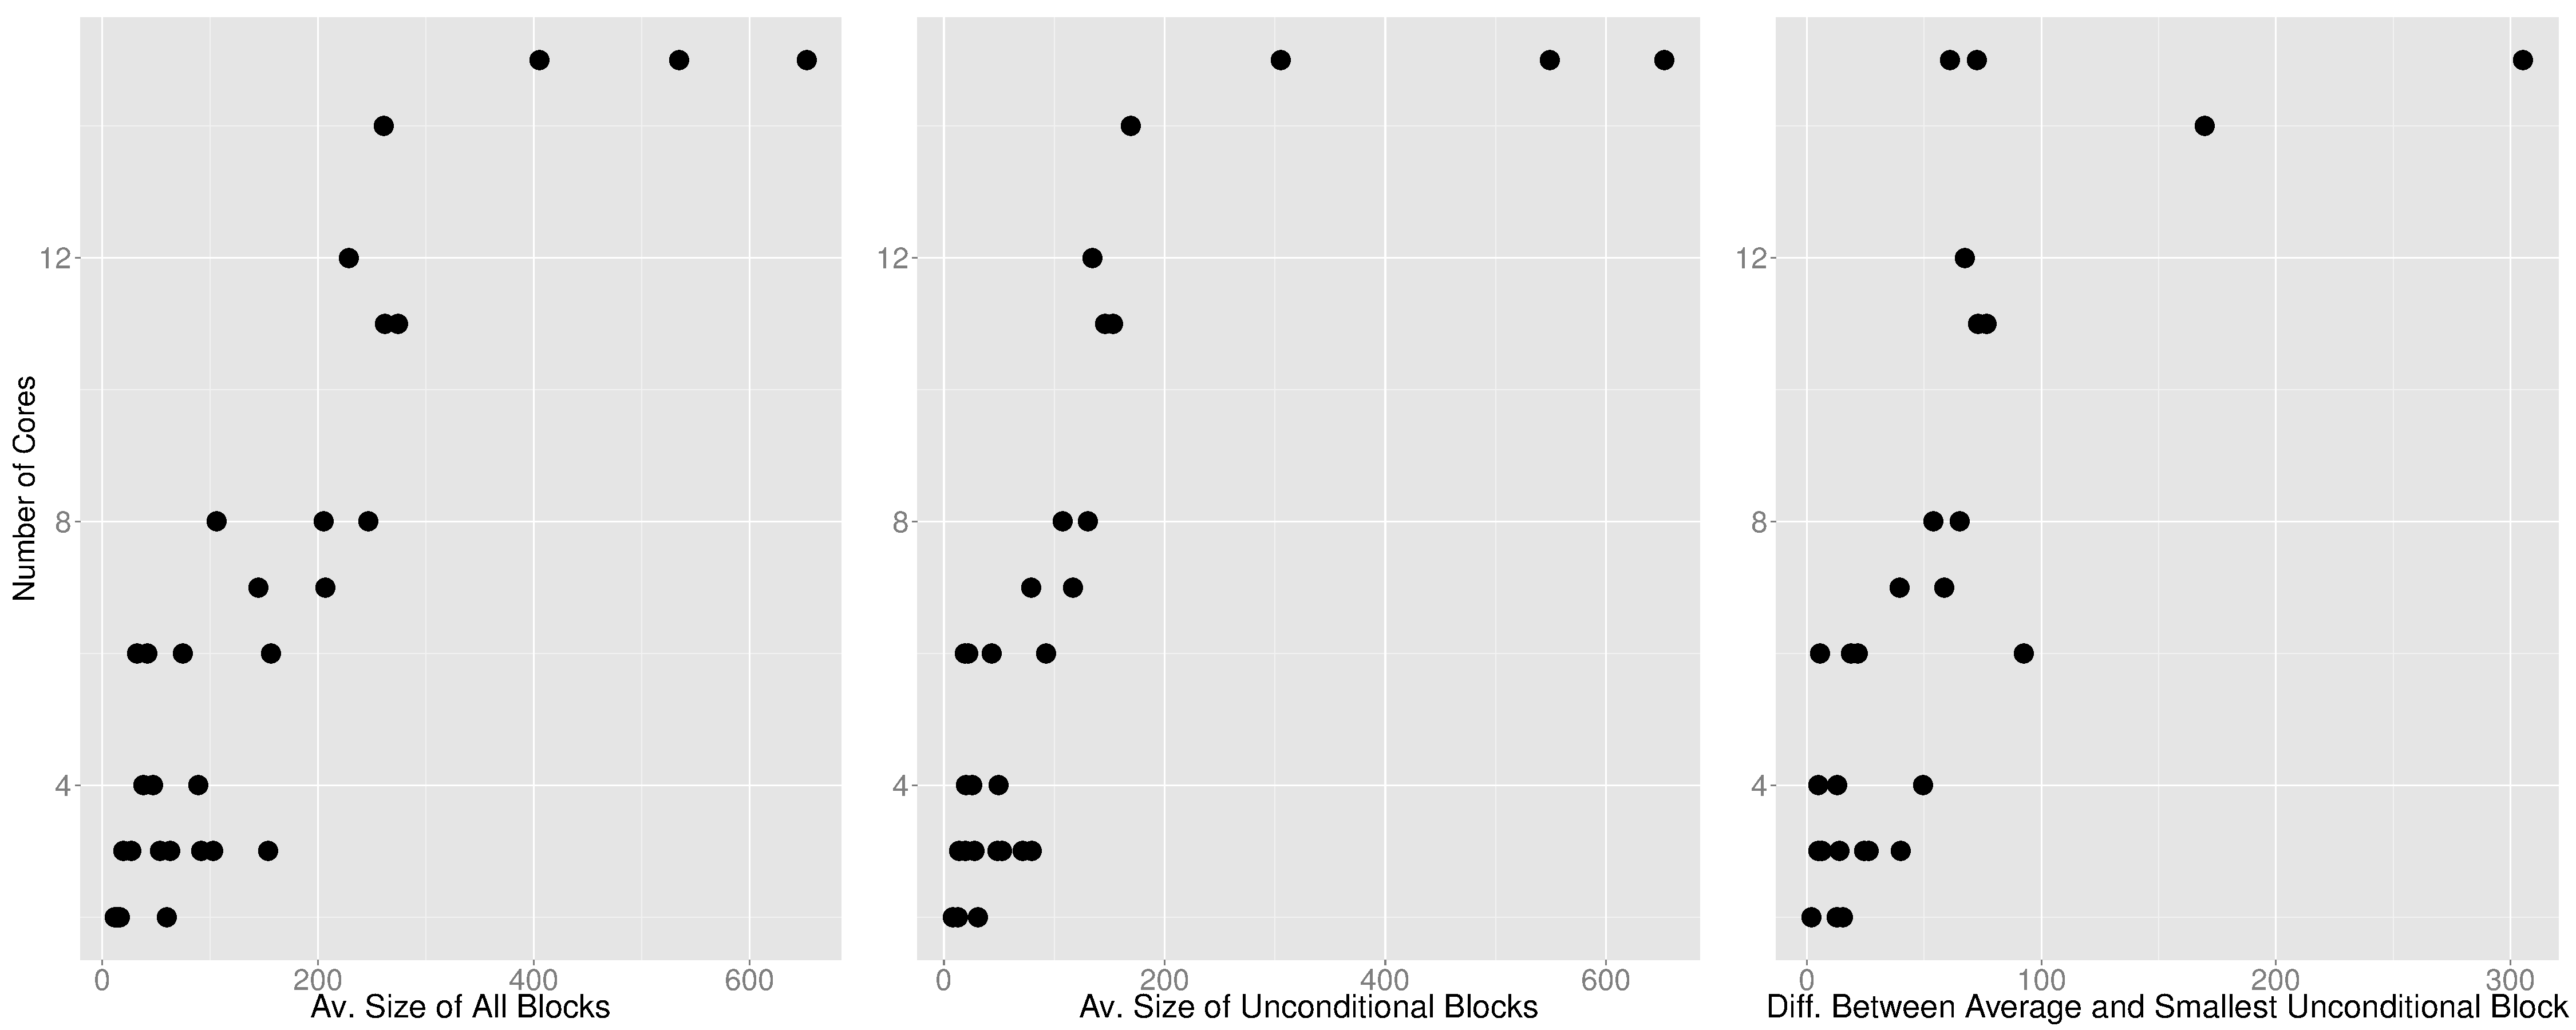
\includegraphics[width=1\textwidth]{streamit-paper/graphics/lineargraphs.pdf}
  \caption{Optimal number of cores in relation to the three highest correlating features. The maximum number of cores plateaus on the right hand side as this is the maximum possible amount.}\label{fig:maxav}
\end{figure}

\subsubsection{Linear Regression Model}
Given that the optimal number of cores highly correlates with a few features, a linear regression is a natural choice to predict the best number of threads.
Figures~\ref{fig:maxav} represent how the first three highest correlating values affect the optimal number of cores for a single-working-thread.
This figure is obtained by finding the best number of cores for the single-working-threaded version of each of the StreamIt benchmarks whilst varying the amount of loop unrolling.
It is important to note that the reason the points in the top right corner appear to converge at 15 cores is due to the fact that no more than 15 cores can be fused.
Overall, Figure~\ref{fig:maxav} shows that StreamIt applications with large unconditionally executed blocks will require large compositions.




\section{Results}
This section describes the performance achieved by the model when predicting the number of threads and core composition to use for each of the StreamIt benchmarks and compares it to the optimal solution found when exploring the space.

\begin{figure}[t]
    \centering
    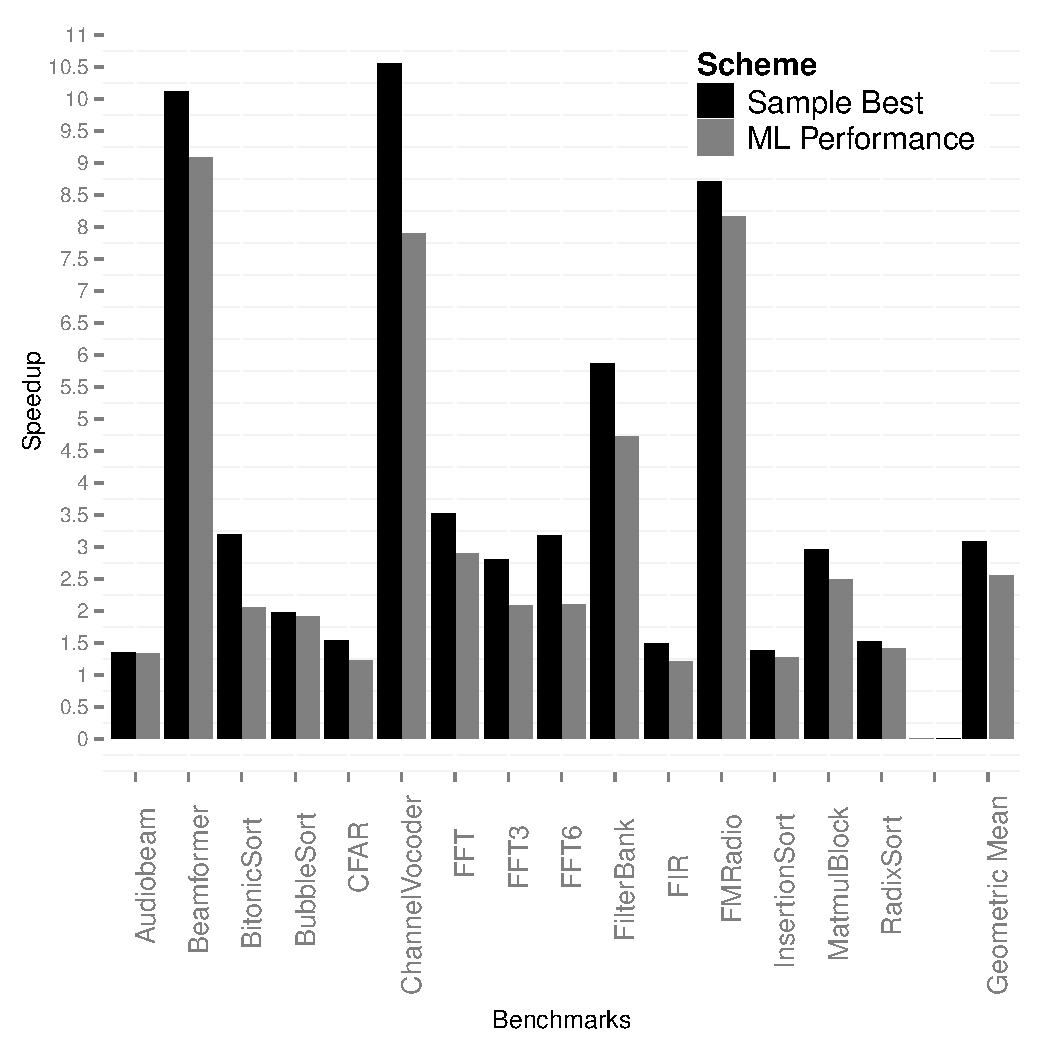
\includegraphics[width=0.7\textwidth]{streamit-paper/graphics/results.pdf}
    \caption{Performance of the machine learning model against the best execution from random sampling. The baseline for the speedup measurement is single core, single thread execution using O2 compiler optimisations. Higher is better.}\label{fig:results}
\end{figure}

\subsection{Machine Learning Model Evaluation Methodology}

Leave-one-out cross-validation is used for testing the linear model.
This means that when testing the model on one application, this application is removed from the training set, the model is trained with the remaining application and finally the model is tested on the application; this process is repeated for each application.
This is standard methodology in the machine-learning community ensuring that the training data is never used for testing.
For the kNN model, the training data consists of all the generated synthetic benchmarks and it is only tested on the real StreamIt applications as they are not used for training.
To obtain the speedup the performance of the machine learning based result are compared to the best from the sample space to running the StreamIt benchmark on a single core, single thread, using O2 compiler optimisations. 

\subsection{Evaluation}

Figure~\ref{fig:results} compares the performance of the machine-learning model and the best performance from the sample space.
As explained in the earlier section, the sampled best is drawn from a sample size of 1,316 combinations of core compositions and thread partitions for each application when possible.
The baseline is the original StreamIt application running with one thread and one core with O2 optimisations on the dynamic multicore processor.
The average speedup obtained through the machine learning model is 2.6 compared to the baseline, this is only 16\% smaller than the average of the best found, which is a speedup of 3.1.
These results are positive as it means the model's results are at least within 16\% of the total best.

As can been seen in Figure~\ref{fig:results} the largest performance penalty resides in the performance of \bench{ChannelVocoder}.
Table~\ref{tab:summary} presents the actual configuration found for the best sampled point and the machine learning model prediction.
Each column represent a different threads and the number in the cell represents the number of core associated with that thread.
For ~\bench{ChannelVocoder} the model predicts only 8 threads rather than the optimal 13.
Referring back to Figure~\ref{fig:threadtrend} and Figure~\ref{fig:overviewhist} from Section~\ref{sec:streamit:dse} \bench{ChannelVocoder} always performs better when adding more threads rather than increasing the size of a core composition.
This is the cause of the performance penalty, for ~\bench{ChannelVocoder} it is more important to allocate a higher number of threads rather than compose cores.
Aside from this case, the machine learning model obtains similar speedups to the best sample.

\begin{table*}[t]
\centering
\resizebox{0.75\textwidth}{!}{\begin{minipage}{0.5\textwidth}
  \small
  \hspace{-5em}
 \begin{tabular} { | l | l | l | l | l | l | l | l | l | l |l| }
    \hline
      & \textbf{1} & \textbf{2} & \textbf{3} & \textbf{4} & \textbf{5} & \textbf{6} & \textbf{7} & \textbf{8} & \textbf{9} & \textbf{10} \\ \hline
    B Audiobeam & 3 & 2 & \cellcolor[gray]{0.3}& \cellcolor[gray]{0.3}& \cellcolor[gray]{0.3}& \cellcolor[gray]{0.3}& \cellcolor[gray]{0.3}& \cellcolor[gray]{0.3}& \cellcolor[gray]{0.3}& \cellcolor[gray]{0.3} \\ \hline 
    M Audiobeam & 2 & 3 & \cellcolor[gray]{0.3}& \cellcolor[gray]{0.3}& \cellcolor[gray]{0.3} & \cellcolor[gray]{0.3}& \cellcolor[gray]{0.3}& \cellcolor[gray]{0.3}& \cellcolor[gray]{0.3}& \cellcolor[gray]{0.3}\\ \hline\hline
    B Beamformer & 1 & 4 & 2 & 4 & 4& \cellcolor[gray]{0.3}& \cellcolor[gray]{0.3}& \cellcolor[gray]{0.3}& \cellcolor[gray]{0.3}& \cellcolor[gray]{0.3} \\ \hline 
    M Beamformer & 6 & 4 & 4& \cellcolor[gray]{0.3}& \cellcolor[gray]{0.3}& \cellcolor[gray]{0.3}& \cellcolor[gray]{0.3}& \cellcolor[gray]{0.3}& \cellcolor[gray]{0.3}& \cellcolor[gray]{0.3} \\ \hline\hline
    B BitonicSort & 3 & 2 & 2 & 2 & \cellcolor[gray]{0.3}& \cellcolor[gray]{0.3}& \cellcolor[gray]{0.3}& \cellcolor[gray]{0.3}& \cellcolor[gray]{0.3}& \cellcolor[gray]{0.3}  \\ \hline
    M BitonicSort & 1 & 2 & 2 & 1 & 2 & 2 & 2 & \cellcolor[gray]{0.3}& \cellcolor[gray]{0.3}& \cellcolor[gray]{0.3} \\ \hline\hline
    B BubbleSort & 3 & 3& \cellcolor[gray]{0.3} & \cellcolor[gray]{0.3} & \cellcolor[gray]{0.3}& \cellcolor[gray]{0.3}& \cellcolor[gray]{0.3}& \cellcolor[gray]{0.3}& \cellcolor[gray]{0.3}& \cellcolor[gray]{0.3} \\ \hline
    M BubbleSort & 2 & \cellcolor[gray]{0.3} & \cellcolor[gray]{0.3} & \cellcolor[gray]{0.3} & \cellcolor[gray]{0.3}& \cellcolor[gray]{0.3}& \cellcolor[gray]{0.3}& \cellcolor[gray]{0.3}& \cellcolor[gray]{0.3}& \cellcolor[gray]{0.3} \\ \hline\hline
    B CFAR & 3 & 2 & \cellcolor[gray]{0.3} & \cellcolor[gray]{0.3} & \cellcolor[gray]{0.3}& \cellcolor[gray]{0.3}& \cellcolor[gray]{0.3}& \cellcolor[gray]{0.3}& \cellcolor[gray]{0.3}& \cellcolor[gray]{0.3} \\ \hline 
    M CFAR & 2 & 2  & 1  & 2 & \cellcolor[gray]{0.3}& \cellcolor[gray]{0.3}& \cellcolor[gray]{0.3}& \cellcolor[gray]{0.3}& \cellcolor[gray]{0.3}& \cellcolor[gray]{0.3} \\ \hline\hline
    B ChannelVoc.& 4 & 1 & 1 & 1 & 1 & 1 & 2 & 1 & 1 & 1 \\ \hline 
    M ChannelVoc.& 2 & 2 & 1 & 2 & 2& 2 & 2& \cellcolor[gray]{0.3}& \cellcolor[gray]{0.3}& \cellcolor[gray]{0.3} \\ \hline\hline
    B FIR & 3 & 2 &\cellcolor[gray]{0.3}&\cellcolor[gray]{0.3}&\cellcolor[gray]{0.3}&\cellcolor[gray]{0.3}&\cellcolor[gray]{0.3}&\cellcolor[gray]{0.3}&\cellcolor[gray]{0.3}&\cellcolor[gray]{0.3}\\ \hline
    M FIR & 2 & 2&\cellcolor[gray]{0.3}&\cellcolor[gray]{0.3}&\cellcolor[gray]{0.3}&\cellcolor[gray]{0.3}&\cellcolor[gray]{0.3}&\cellcolor[gray]{0.3}&\cellcolor[gray]{0.3}&\cellcolor[gray]{0.3}\\ \hline\hline
    \end{tabular}
  \end{minipage}	\hfill
  \hspace{1em}
\begin{minipage}{0.5\textwidth}

	 \begin{tabular} { | l | l | l | l | l | l | l |}
    \hline
      & \textbf{1} & \textbf{2} & \textbf{3} & \textbf{4} & \textbf{5} & \textbf{6}  \\ \hline

	B FFT & 3 & 3 & 5 & \cellcolor[gray]{0.3}& \cellcolor[gray]{0.3}& \cellcolor[gray]{0.3} \\ \hline
    M FFT & 6& 5 & 2& \cellcolor[gray]{0.3}& \cellcolor[gray]{0.3}& \cellcolor[gray]{0.3}  \\ \hline\hline
    B FFT3 & 3 & 2 & 2& \cellcolor[gray]{0.3}& \cellcolor[gray]{0.3}& \cellcolor[gray]{0.3} \\ \hline 
    M FFT3 & 3 & 2 & 3 & 3& 3& 3 \\ \hline\hline
    B FFT6 & 7 & 8& \cellcolor[gray]{0.3}& \cellcolor[gray]{0.3}& \cellcolor[gray]{0.3}& \cellcolor[gray]{0.3}\\ \hline
    M FFT6& 14 & \cellcolor[gray]{0.3}& \cellcolor[gray]{0.3}& \cellcolor[gray]{0.3}& \cellcolor[gray]{0.3}& \cellcolor[gray]{0.3} \\ \hline\hline
    B FilterBank & 4 & 5 & 6& \cellcolor[gray]{0.3}& \cellcolor[gray]{0.3}& \cellcolor[gray]{0.3} \\ \hline
    M FilterBank & 4 & 5 & \cellcolor[gray]{0.3} & \cellcolor[gray]{0.3}& \cellcolor[gray]{0.3}& \cellcolor[gray]{0.3}\\ \hline\hline
    B FMRadio & 7 & 6 & \cellcolor[gray]{0.3}& \cellcolor[gray]{0.3}& \cellcolor[gray]{0.3}& \cellcolor[gray]{0.3}\\ \hline
    M FMRadio & 7 & 4 & \cellcolor[gray]{0.3} & \cellcolor[gray]{0.3}& \cellcolor[gray]{0.3}& \cellcolor[gray]{0.3} \\ \hline\hline
    B InsertionSort & 3 & 2& \cellcolor[gray]{0.3}& \cellcolor[gray]{0.3}& \cellcolor[gray]{0.3}& \cellcolor[gray]{0.3} \\ \hline
    M InsertionSort & 3 & \cellcolor[gray]{0.3}& \cellcolor[gray]{0.3}& \cellcolor[gray]{0.3}& \cellcolor[gray]{0.3}& \cellcolor[gray]{0.3}\\ \hline\hline
    B MatmulBlock & 3 & 4 & 6 & 2 & \cellcolor[gray]{0.3} & \cellcolor[gray]{0.3}\\ \hline
    M MatmulBlock & 4 & 4 & \cellcolor[gray]{0.3}& \cellcolor[gray]{0.3}& \cellcolor[gray]{0.3}& \cellcolor[gray]{0.3}\\ \hline\hline
    B RadixSort & 3 & 3& \cellcolor[gray]{0.3}& \cellcolor[gray]{0.3}& \cellcolor[gray]{0.3}& \cellcolor[gray]{0.3}\\ \hline
    M RadixSort & 2 & 2& \cellcolor[gray]{0.3}& \cellcolor[gray]{0.3}& \cellcolor[gray]{0.3}& \cellcolor[gray]{0.3}\\ \hline
    
 \end{tabular}
  \end{minipage}}
  \caption{Number of Threads and Cores used for Best of Sample Space and Machine Learning Model.}\label{tab:summary}

\end{table*}

 \subsection{Summary}

This section has demonstrated that it is possible to build a machine-learning model that achieves high level of performance using simple source code static features.
In many applications, the model even comes very close to the best from the sampled space, showing that the features used by the model contain enough information to inform the model about the best decision.

\vspace{5mm}


\appendix
\section{Appendix Title}

This is the text of the appendix, if you need one.

\acks

Acknowledgments, if needed.

% We recommend abbrvnat bibliography style.

\bibliographystyle{abbrvnat}
\bibliography{references}


% The bibliography should be embedded for final submission.

\begin{thebibliography}{}
\softraggedright
\providecommand{\natexlab}[1]{#1}
\providecommand{\url}[1]{\texttt{#1}}
\expandafter\ifx\csname urlstyle\endcsname\relax
  \providecommand{\doi}[1]{doi: #1}\else
  \providecommand{\doi}{doi: \begingroup \urlstyle{rm}\Url}\fi

\bibitem[Auerbach et~al.(2012)Auerbach, Bacon, Burcea, Cheng, Fink, Rabbah, and
  Shukla]{auerbach2012lime}
J.~Auerbach, D.~Bacon, I.~Burcea, P.~Cheng, S.~Fink, R.~Rabbah, and S.~Shukla.
\newblock A compiler and runtime for heterogeneous computing.
\newblock In \emph{Design Automation Conference (DAC), 2012 49th
  ACM/EDAC/IEEE}, pages 271--276, June 2012.

\bibitem[Buck et~al.(2004)Buck, Foley, Horn, Sugerman, Fatahalian, Houston, and
  Hanrahan]{buck2004brook}
I.~Buck, T.~Foley, D.~Horn, J.~Sugerman, K.~Fatahalian, M.~Houston, and
  P.~Hanrahan.
\newblock Brook for gpus: Stream computing on graphics hardware.
\newblock In \emph{ACM SIGGRAPH 2004 Papers}, SIGGRAPH '04, pages 777--786, New
  York, NY, USA, 2004. ACM.
\newblock \doi{10.1145/1186562.1015800}.
\newblock URL \url{http://doi.acm.org/10.1145/1186562.1015800}.

\bibitem[Chen et~al.(2005)Chen, Gordon, Thies, Zwicker, Pulli, and
  Durand]{chen2005rawstream}
J.~Chen, M.~I. Gordon, W.~Thies, M.~Zwicker, K.~Pulli, and F.~Durand.
\newblock A reconfigurable architecture for load-balanced rendering.
\newblock In \emph{Proceedings of the ACM SIGGRAPH/EUROGRAPHICS Conference on
  Graphics Hardware}, HWWS '05, pages 71--80, New York, NY, USA, 2005. ACM.
\newblock ISBN 1-59593-086-8.
\newblock \doi{10.1145/1071866.1071878}.
\newblock URL \url{http://doi.acm.org/10.1145/1071866.1071878}.

\bibitem[Gordon et~al.(2006)Gordon, Thies, and
  Amarasinghe]{gordon2006coarsegrainstream}
M.~I. Gordon, W.~Thies, and S.~Amarasinghe.
\newblock Exploiting coarse-grained task, data, and pipeline parallelism in
  stream programs.
\newblock \emph{SIGARCH Comput. Archit. News}, 34\penalty0 (5):\penalty0
  151--162, Oct. 2006.
\newblock ISSN 0163-5964.
\newblock \doi{10.1145/1168919.1168877}.
\newblock URL \url{http://doi.acm.org/10.1145/1168919.1168877}.

\bibitem[Hagiescu et~al.(2009)Hagiescu, Wong, Bacon, and
  Rabbah]{hagiescu2009fpgafolding}
A.~Hagiescu, W.-F. Wong, D.~F. Bacon, and R.~Rabbah.
\newblock A computing origami: Folding streams in fpgas.
\newblock In \emph{Proceedings of the 46th Annual Design Automation
  Conference}, DAC '09, pages 282--287, New York, NY, USA, 2009. ACM.
\newblock ISBN 978-1-60558-497-3.
\newblock \doi{10.1145/1629911.1629987}.
\newblock URL \url{http://doi.acm.org/10.1145/1629911.1629987}.

\bibitem[Hill and Marty(2008)]{mark2008amdahl}
M.~D. Hill and M.~R. Marty.
\newblock Amdahl's law in the multicore era.
\newblock \emph{Computer}, 41\penalty0 (7):\penalty0 33--38, 2008.
\newblock ISSN 0018-9162.
\newblock \doi{http://doi.ieeecomputersociety.org/10.1109/MC.2008.209}.

\bibitem[Ipek et~al.(2007)Ipek, Kirman, Kirman, and
  Martinez]{ipek2007corefusion}
E.~Ipek, M.~Kirman, N.~Kirman, and J.~F. Martinez.
\newblock Core fusion: Accommodating software diversity in chip
  multiprocessors.
\newblock \emph{SIGARCH Comput. Archit. News}, 35\penalty0 (2):\penalty0
  186--197, June 2007.
\newblock ISSN 0163-5964.
\newblock \doi{10.1145/1273440.1250686}.
\newblock URL \url{http://doi.acm.org/10.1145/1273440.1250686}.

\bibitem[Kim et~al.(2007)Kim, Sethumadhavan, Govindan, Ranganathan, Gulati,
  Burger, and Keckler]{kim2007composableproc}
C.~Kim, S.~Sethumadhavan, M.~S. Govindan, N.~Ranganathan, D.~Gulati, D.~Burger,
  and S.~W. Keckler.
\newblock Composable lightweight processors.
\newblock In \emph{Proceedings of the 40th Annual IEEE/ACM International
  Symposium on Microarchitecture}, MICRO 40, pages 381--394, Washington, DC,
  USA, 2007. IEEE Computer Society.
\newblock ISBN 0-7695-3047-8.
\newblock \doi{10.1109/MICRO.2007.10}.
\newblock URL \url{http://dx.doi.org/10.1109/MICRO.2007.10}.

\bibitem[Kudlur and Mahlke(2008)]{kudlur2008orchestratingstreamprog}
M.~Kudlur and S.~Mahlke.
\newblock Orchestrating the execution of stream programs on multicore
  platforms.
\newblock \emph{SIGPLAN Not.}, 43\penalty0 (6):\penalty0 114--124, June 2008.
\newblock ISSN 0362-1340.
\newblock \doi{10.1145/1379022.1375596}.
\newblock URL \url{http://doi.acm.org/10.1145/1379022.1375596}.

\bibitem[Nagatsuka et~al.(2011)Nagatsuka, Sakaguchi, Matsumura, and
  Kise]{nagatsuka2011coresymphony}
T.~Nagatsuka, Y.~Sakaguchi, T.~Matsumura, and K.~Kise.
\newblock Coresymphony: An efficient reconfigurable multi-core architecture.
\newblock \emph{SIGARCH Comput. Archit. News}, 39\penalty0 (4):\penalty0
  32--37, Dec. 2011.
\newblock ISSN 0163-5964.
\newblock \doi{10.1145/2082156.2082165}.
\newblock URL \url{http://doi.acm.org/10.1145/2082156.2082165}.

\bibitem[Putnam et~al.(2011)Putnam, Smith, and Burger]{putnam2010dynamicvece2}
A.~Putnam, A.~Smith, and D.~Burger.
\newblock Dynamic vectorization in the e2 dynamic multicore architecture.
\newblock \emph{SIGARCH Comput. Archit. News}, 38\penalty0 (4):\penalty0
  27--32, Jan. 2011.
\newblock ISSN 0163-5964.
\newblock \doi{10.1145/1926367.1926373}.
\newblock URL \url{http://doi.acm.org/10.1145/1926367.1926373}.

\bibitem[R()]{rknn}
R.
\newblock R: K-nearest neighbor.
\newblock URL
  \url{https://stat.ethz.ch/R-manual/R-devel/library/class/html/knn.html}.

\bibitem[Smith et~al.(2006)Smith, Burrill, Gibson, Maher, Nethercote, Yoder,
  Burger, and McKinley]{smith2006compilingedge}
A.~Smith, J.~Burrill, J.~Gibson, B.~Maher, N.~Nethercote, B.~Yoder, D.~Burger,
  and K.~McKinley.
\newblock Compiling for edge architectures.
\newblock In \emph{Code Generation and Optimization, 2006. CGO 2006.
  International Symposium on}, pages 11 pp.--, March 2006.
\newblock \doi{10.1109/CGO.2006.10}.

\bibitem[Suleman et~al.(2009)Suleman, Mutlu, Qureshi, and
  Patt]{suleman2009asymmetric}
M.~A. Suleman, O.~Mutlu, M.~K. Qureshi, and Y.~N. Patt.
\newblock Accelerating critical section execution with asymmetric multi-core
  architectures.
\newblock \emph{SIGPLAN Not.}, 44\penalty0 (3):\penalty0 253--264, Mar. 2009.
\newblock ISSN 0362-1340.
\newblock \doi{10.1145/1508284.1508274}.
\newblock URL \url{http://doi.acm.org/10.1145/1508284.1508274}.

\bibitem[Thies et~al.(2002{\natexlab{a}})Thies, Karczmarek, and
  Amarasinghe]{theis2002streamit}
W.~Thies, M.~Karczmarek, and S.~P. Amarasinghe.
\newblock Streamit: A language for streaming applications.
\newblock In \emph{Proceedings of the 11th International Conference on Compiler
  Construction}, CC '02, pages 179--196, London, UK, UK, 2002{\natexlab{a}}.
  Springer-Verlag.
\newblock ISBN 3-540-43369-4.
\newblock URL \url{http://dl.acm.org/citation.cfm?id=647478.727935}.

\bibitem[Thies et~al.(2002{\natexlab{b}})Thies, Karczmarek, Gordon, Maze, Wong,
  Hoffmann, Brown, and Amarasinghe]{theis2002languagegrid}
W.~Thies, M.~Karczmarek, M.~Gordon, D.~Maze, J.~Wong, H.~Hoffmann, M.~Brown,
  and S.~Amarasinghe.
\newblock A common machine language for grid-based architectures.
\newblock \emph{SIGARCH Comput. Archit. News}, 30\penalty0 (3):\penalty0
  13--14, June 2002{\natexlab{b}}.
\newblock ISSN 0163-5964.
\newblock \doi{10.1145/571666.571673}.
\newblock URL \url{http://doi.acm.org/10.1145/571666.571673}.

\bibitem[Waingold et~al.(1997)Waingold, Taylor, Srikrishna, Sarkar, Lee, Lee,
  Kim, Frank, Finch, Barua, Babb, Amarasinghe, and Agarwal]{waingold1997raw}
E.~Waingold, M.~Taylor, D.~Srikrishna, V.~Sarkar, W.~Lee, V.~Lee, J.~Kim,
  M.~Frank, P.~Finch, R.~Barua, J.~Babb, S.~Amarasinghe, and A.~Agarwal.
\newblock Baring it all to software: Raw machines.
\newblock \emph{Computer}, 30\penalty0 (9):\penalty0 86--93, Sep 1997.
\newblock ISSN 0018-9162.
\newblock \doi{10.1109/2.612254}.

\bibitem[Wang and O'boyle(2008)]{wang2013partitionstreamit}
Z.~Wang and M.~F.~P. O'boyle.
\newblock Using machine learning to partition streaming programs.
\newblock \emph{ACM Trans. Archit. Code Optim.}, 10\penalty0 (3):\penalty0
  20:1--20:25, Sept. 2008.
\newblock ISSN 1544-3566.
\newblock \doi{10.1145/2512436}.
\newblock URL \url{http://doi.acm.org/10.1145/2512436}.

\bibitem[Watanabe et~al.(2010)Watanabe, Davis, and Wood]{watanabe2010widget}
Y.~Watanabe, J.~D. Davis, and D.~A. Wood.
\newblock Widget: Wisconsin decoupled grid execution tiles.
\newblock \emph{SIGARCH Comput. Archit. News}, 38\penalty0 (3):\penalty0 2--13,
  June 2010.
\newblock ISSN 0163-5964.
\newblock \doi{10.1145/1816038.1815965}.
\newblock URL \url{http://doi.acm.org/10.1145/1816038.1815965}.

\bibitem[Zhou and Wentzlaff(2014)]{zhou2014sharingarch}
Y.~Zhou and D.~Wentzlaff.
\newblock The sharing architecture: Sub-core configurability for iaas clouds.
\newblock \emph{SIGPLAN Not.}, 49\penalty0 (4):\penalty0 559--574, Feb. 2014.
\newblock ISSN 0362-1340.
\newblock \doi{10.1145/2644865.2541950}.
\newblock URL \url{http://doi.acm.org/10.1145/2644865.2541950}.


\end{thebibliography}



\end{document}

%                       Revision History
%                       -------- -------
%  Date         Person  Ver.    Change
%  ----         ------  ----    ------

%  2013.06.29   TU      0.1--4  comments on permission/copyright notices

